\documentclass[11pt,a4paper]{article}
\usepackage[latin1]{inputenc}
\usepackage{amsmath}
\usepackage{amsfonts}
\usepackage[super,sort&compress,comma]{natbib}
\usepackage{amssymb}
\usepackage{graphicx}
\usepackage{hyperref}
\author{Andrew R. McCluskey,\textit{$^{ab}$}$^{\ddag}$ Adrian Sanchez-Fernandez,\textit{$^{ac}$}$^{\ddag\P}$ \\
Karen J. Edler,\textit{$^{a}$}$^{\ast}$ Stephen C. Parker,\textit{$^{a}$} Andrew J. Jackson,\textit{$^{cd}$} \\
Richard A. Campbell,\textit{$^{ef}$} and Thomas Arnold\textit{$^{abcg}$}$^{\ast}$ \\
 \\
\textit{$^{a}$~Department of Chemistry, University of Bath, Claverton} \\
\textit{Down, Bath, BA2 7AY, UK.} \\
\textit{$^{b}$~Diamond Light Source, Harwell Campus, Didcot, OX11 0DE,} \\
\textit{UK.} \\
\textit{$^{c}$~European Spallation Source, SE-211 00 Lund, Sweden.} \\
\textit{$^{d}$~Department of Physical Chemistry, Lund University,} \\
\textit{SE-211 00 Lund, Sweden.} \\
\textit{$^{e}$~Institut Laue-Langevin, 71 avenue des Martyrs, 38000,} \\
\textit{Grenoble, France.} \\
\textit{$^{f}$~Division of Pharmacy and Optometry, University of} \\
\textit{Manchester, Manchester, M13 9PT, UK.} \\
\textit{$^{g}$~ISIS Neutron and Muon Source, Science and Technology} \\
\textit{Facilities Council, Rutherford Appleton Laboratory, Harwell} \\
\textit{Oxford, Didcot OX11 0QX, UK.} \\
\textit{$^{\P}$~Present address: Department of Food Technology, Lund} \\
\textit{University, SE-211 00 Lund, Sweden}}
\title{ESI for ``Bayesian determination of the effect of a deep eutectic solvent on the structure of lipid monolayers''}
\date{}
\begin{document}

\maketitle
\section{Probability distribution functions}

The two-dimensional probability distribution functions (PDFs) for all parameters and all lipids from the X-ray reflectometry models are given in Figures \ref{fig:dlpc2}-\ref{fig:dmpg5}. The two-dimensional probability distribution functions (PDFs) for all parameters and all lipids from the neutron reflectometry models are given in Figures \ref{fig:dmpcn1}-\ref{fig:dppcn2}.
\begin{figure}[h]
	\centering
	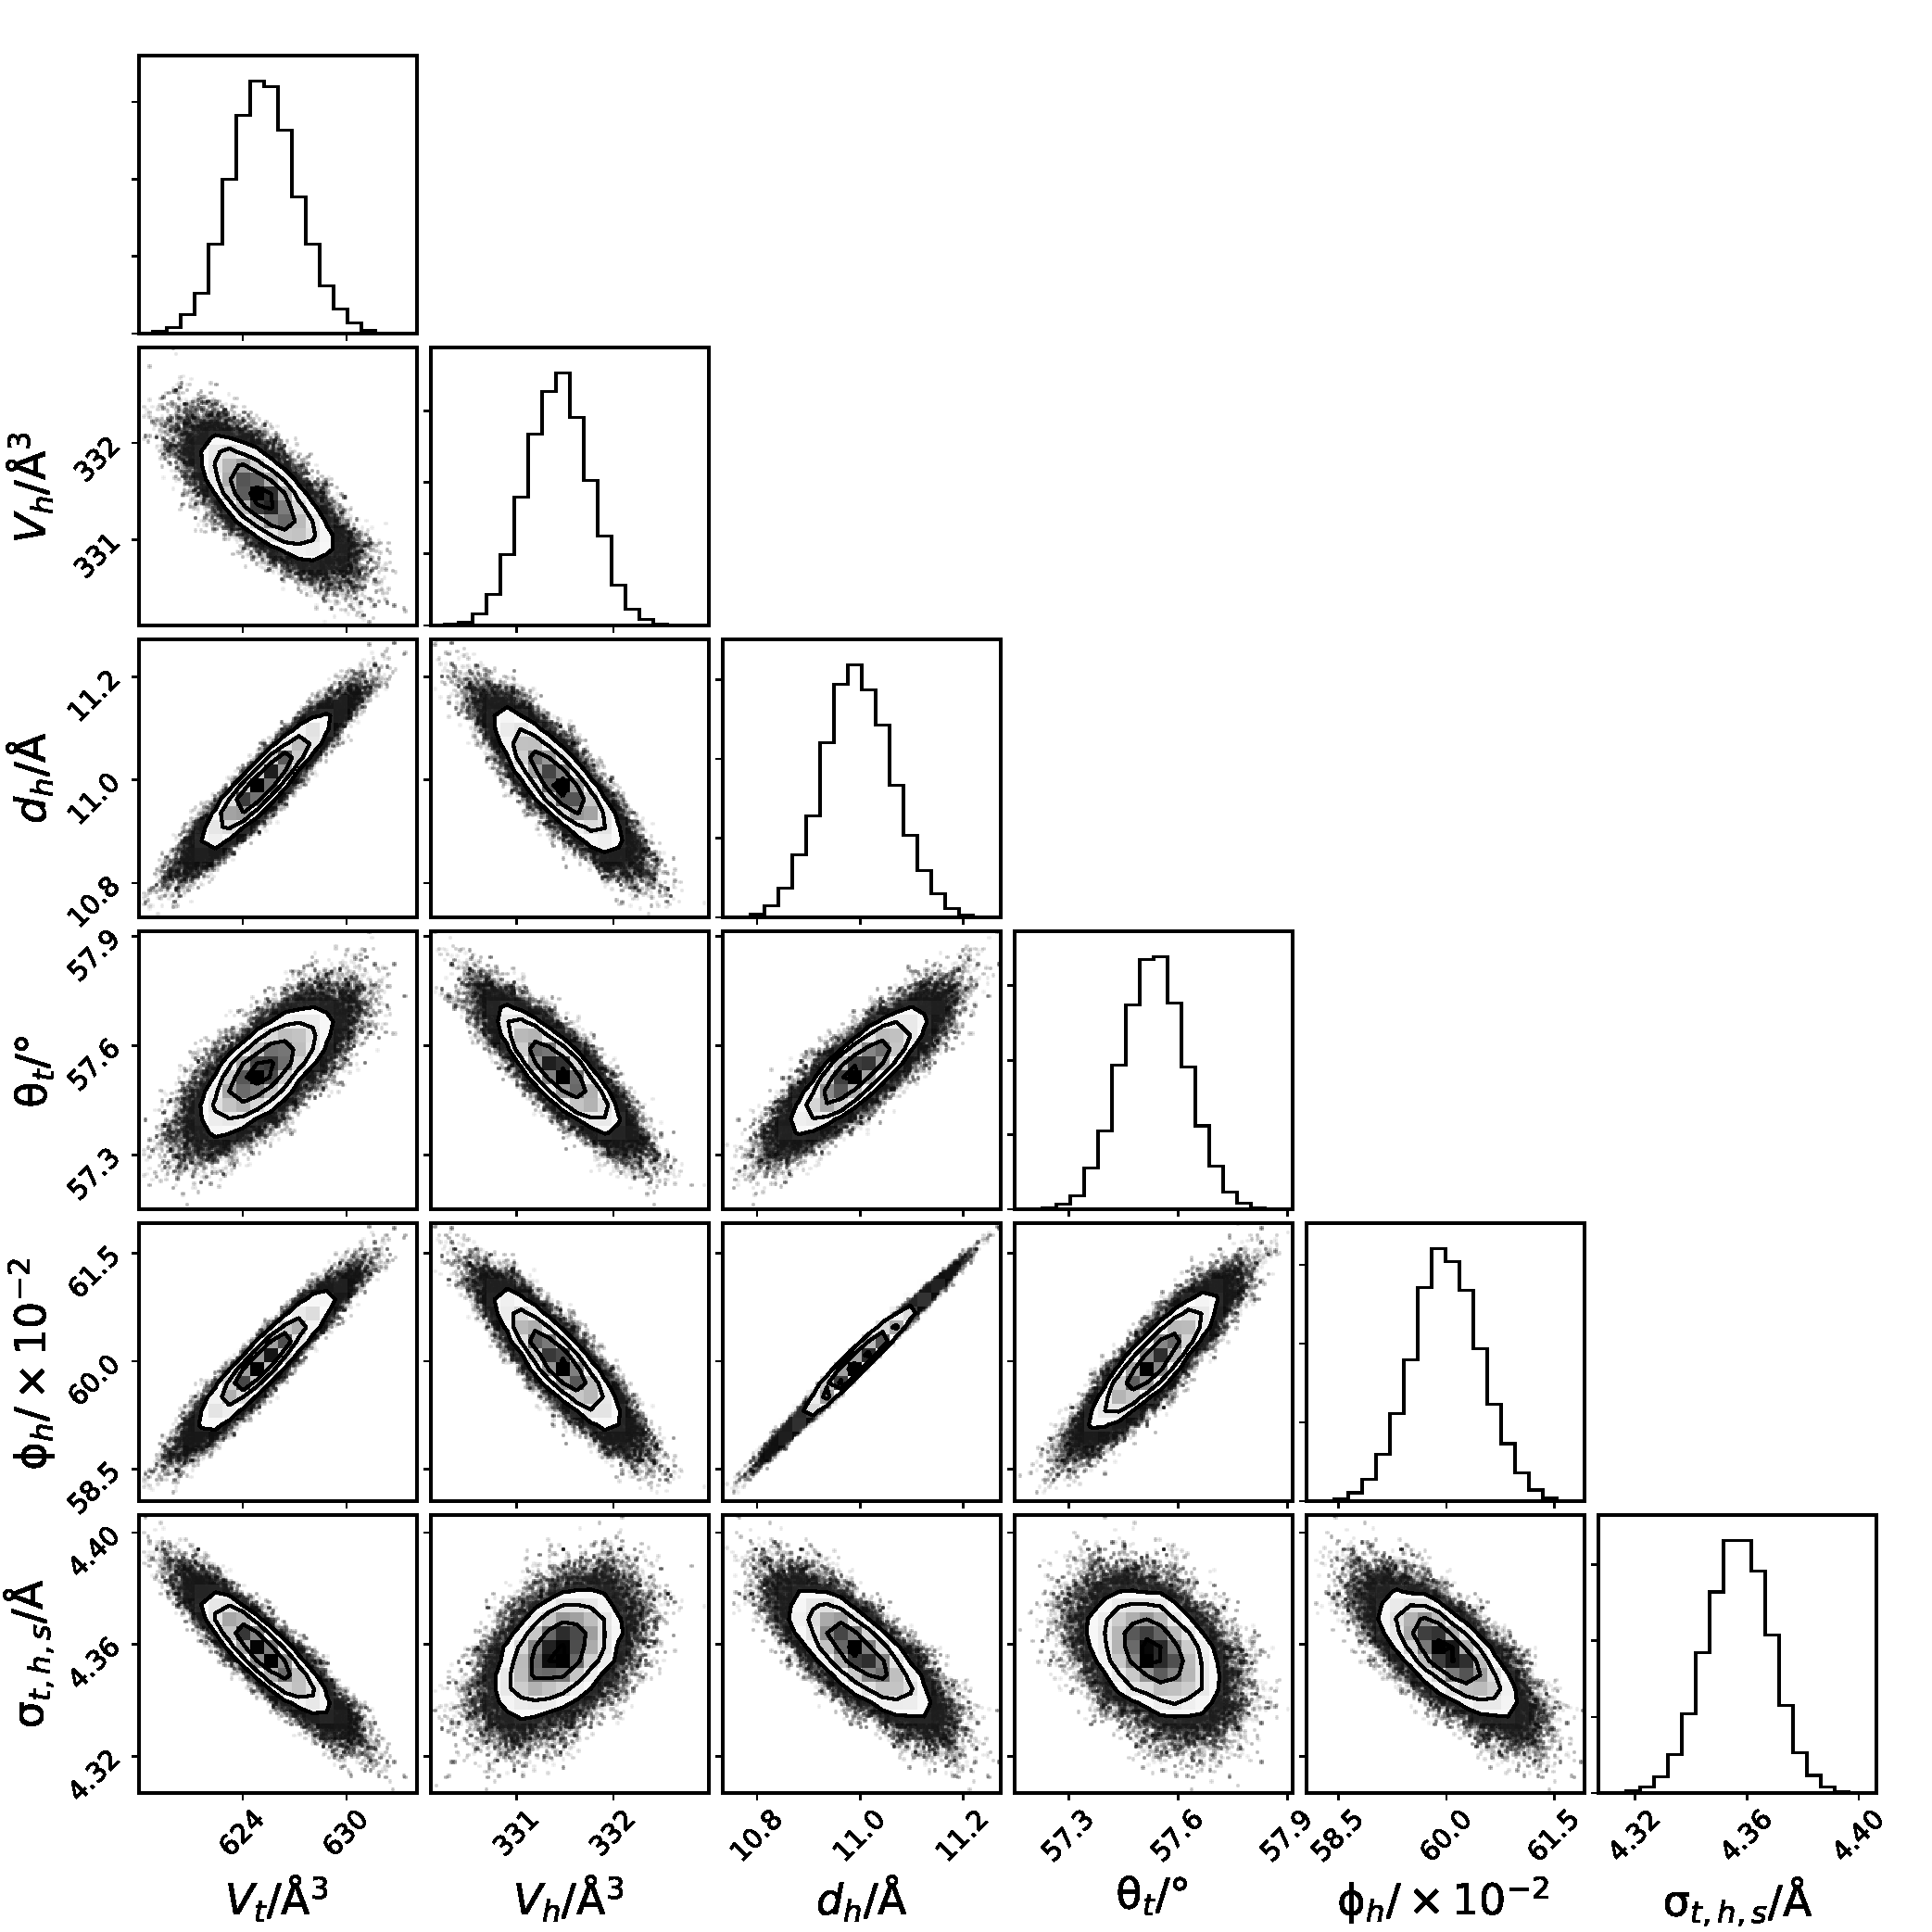
\includegraphics[width=0.50\textwidth]{figures/dlpc2_all_corner}
	\caption{The multi-parameter PDFs for the chemically-relevant model of DLPC X-ray reflectometry data at 20 mNm$^{-1}$. Source: Datasets, figure files and running/plotting scripts are available under CC-BY.\cite{mccluskey_2018}}
	\label{fig:dlpc2}
\end{figure}
\begin{figure}[h]
	\centering
	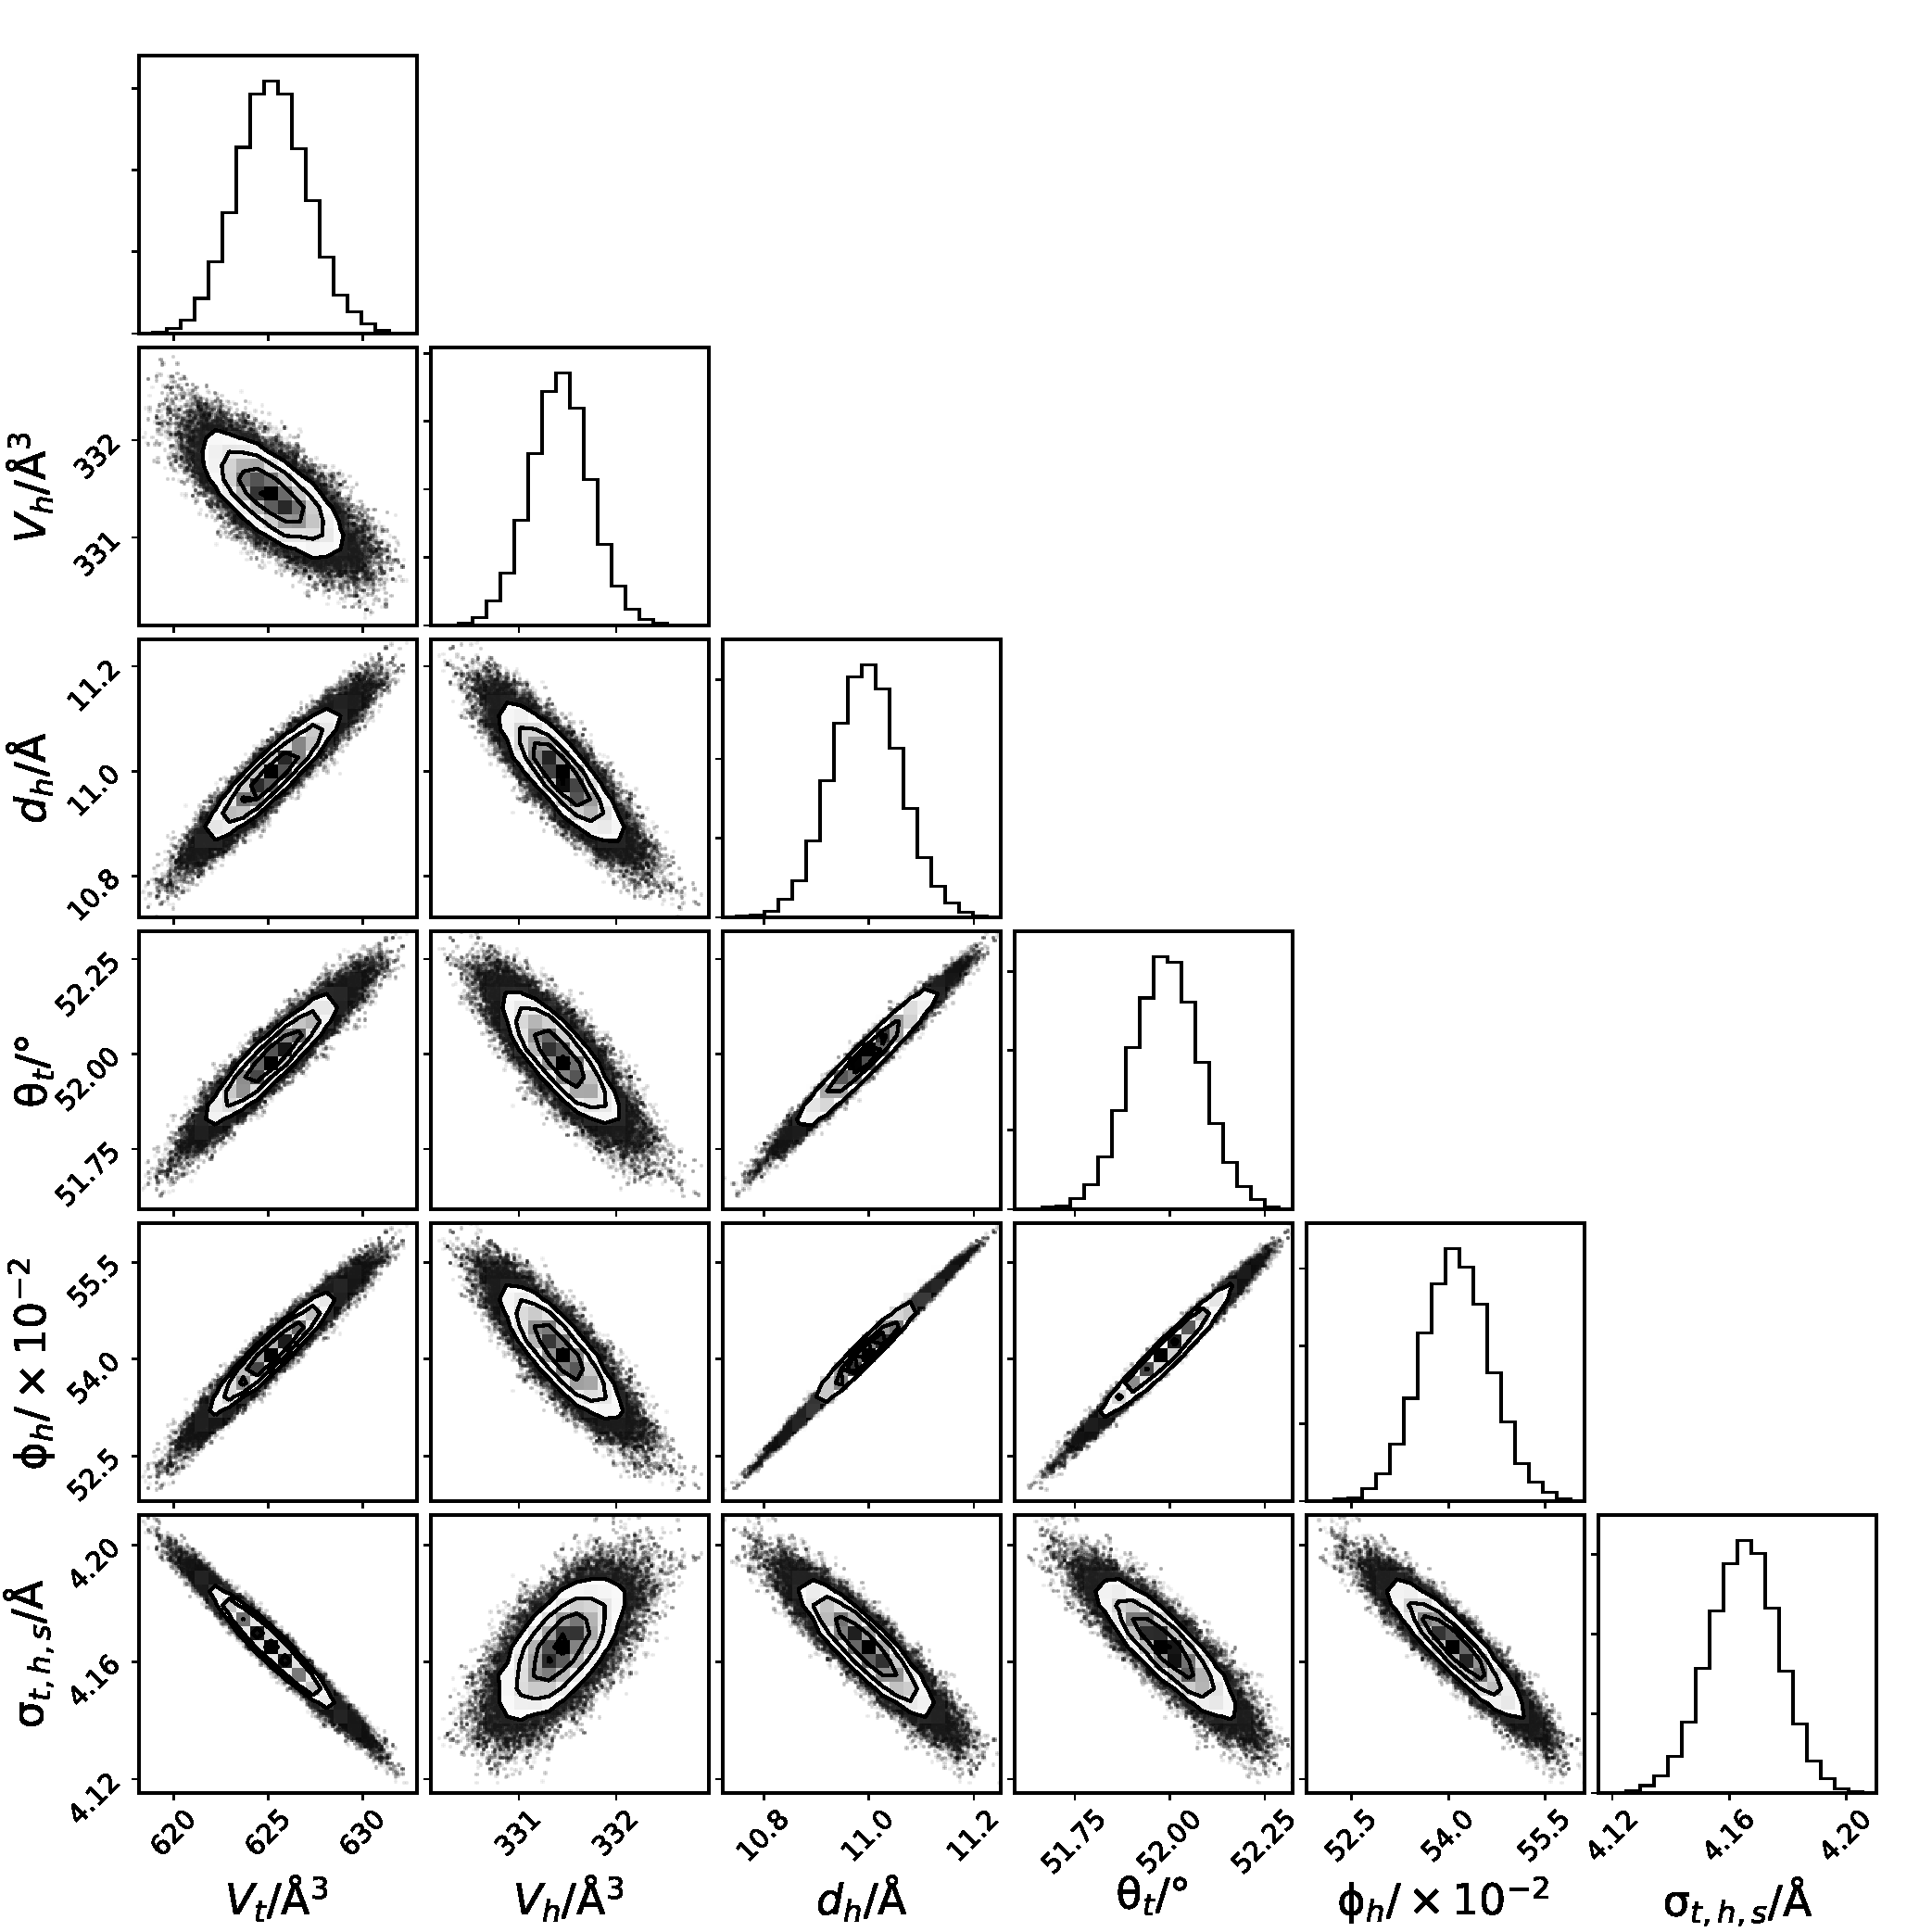
\includegraphics[width=0.50\textwidth]{figures/dlpc3_all_corner}
	\caption{The multi-parameter PDFs for the chemically-relevant model of DLPC X-ray reflectometry data at 25 mNm$^{-1}$. Source: Datasets, figure files and running/plotting scripts are available under CC-BY.\cite{mccluskey_2018}}
	\label{fig:dlpc3}
\end{figure}
\begin{figure}[h]
	\centering
	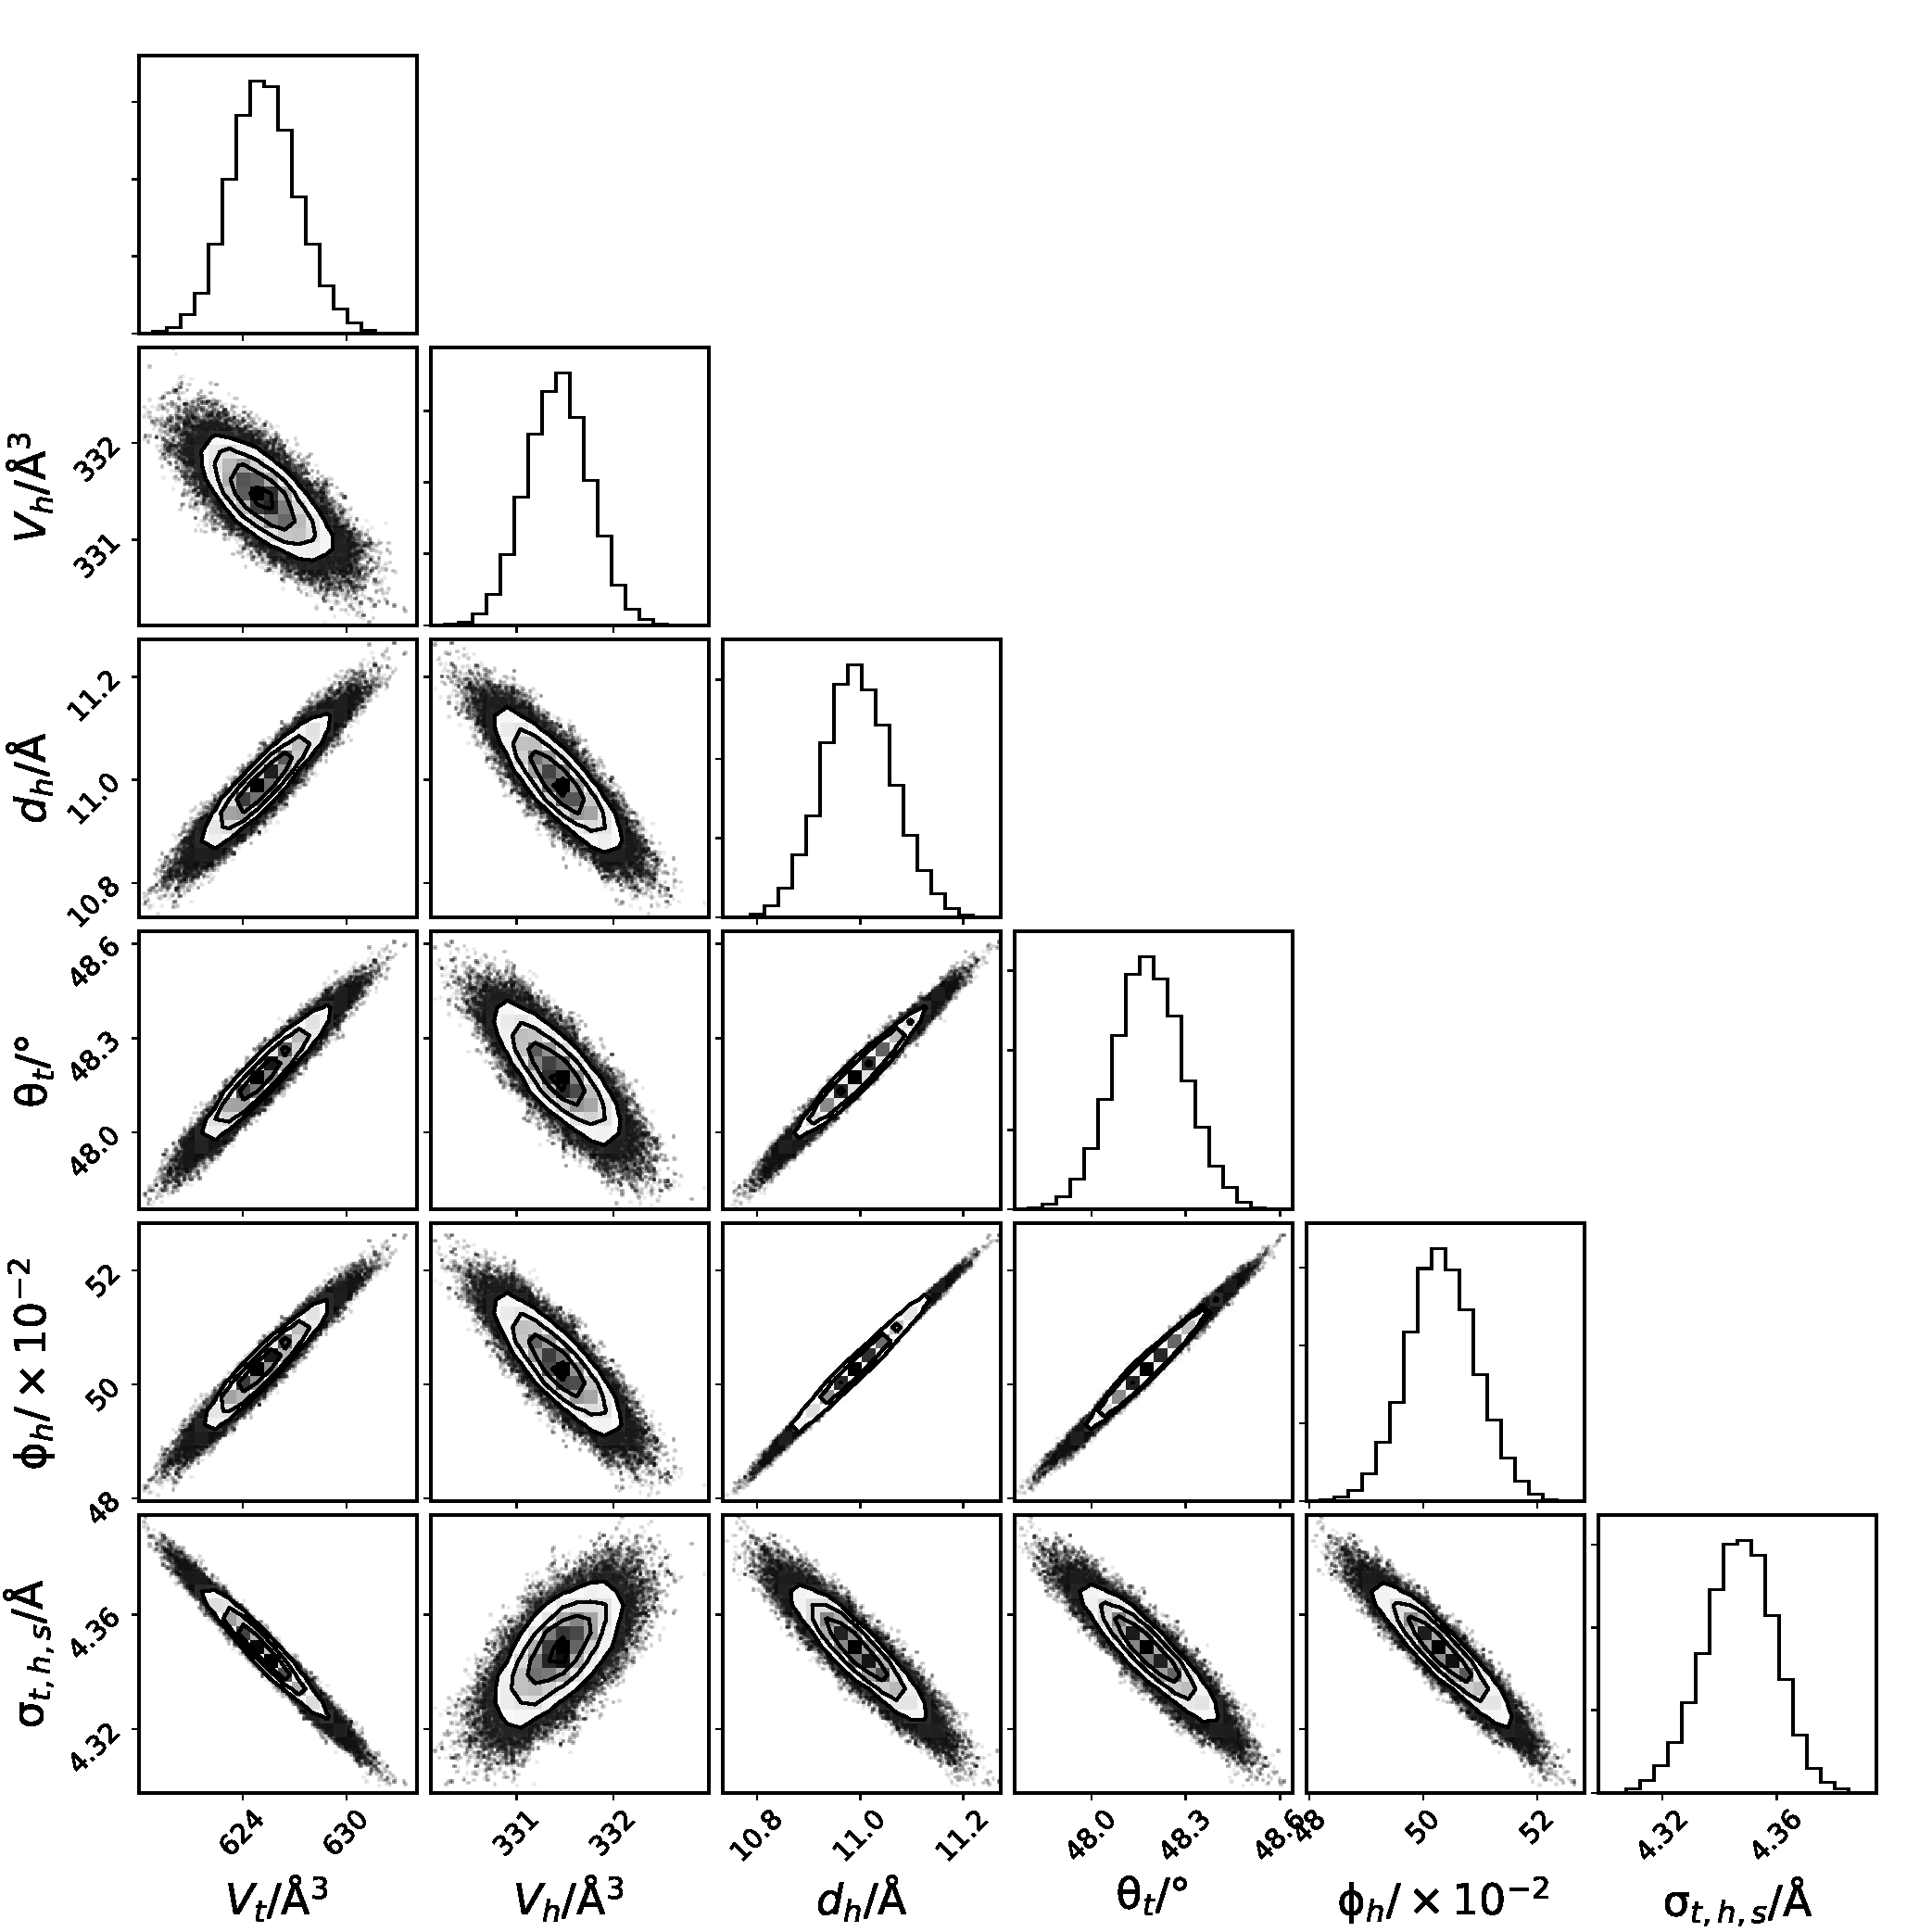
\includegraphics[width=0.50\textwidth]{figures/dlpc4_all_corner}
	\caption{The multi-parameter PDFs for the chemically-relevant model of DLPC X-ray reflectometry data at 30 mNm$^{-1}$. Source: Datasets, figure files and running/plotting scripts are available under CC-BY.\cite{mccluskey_2018}}
	\label{fig:dlpc4}
\end{figure}
\begin{figure}
	\centering
	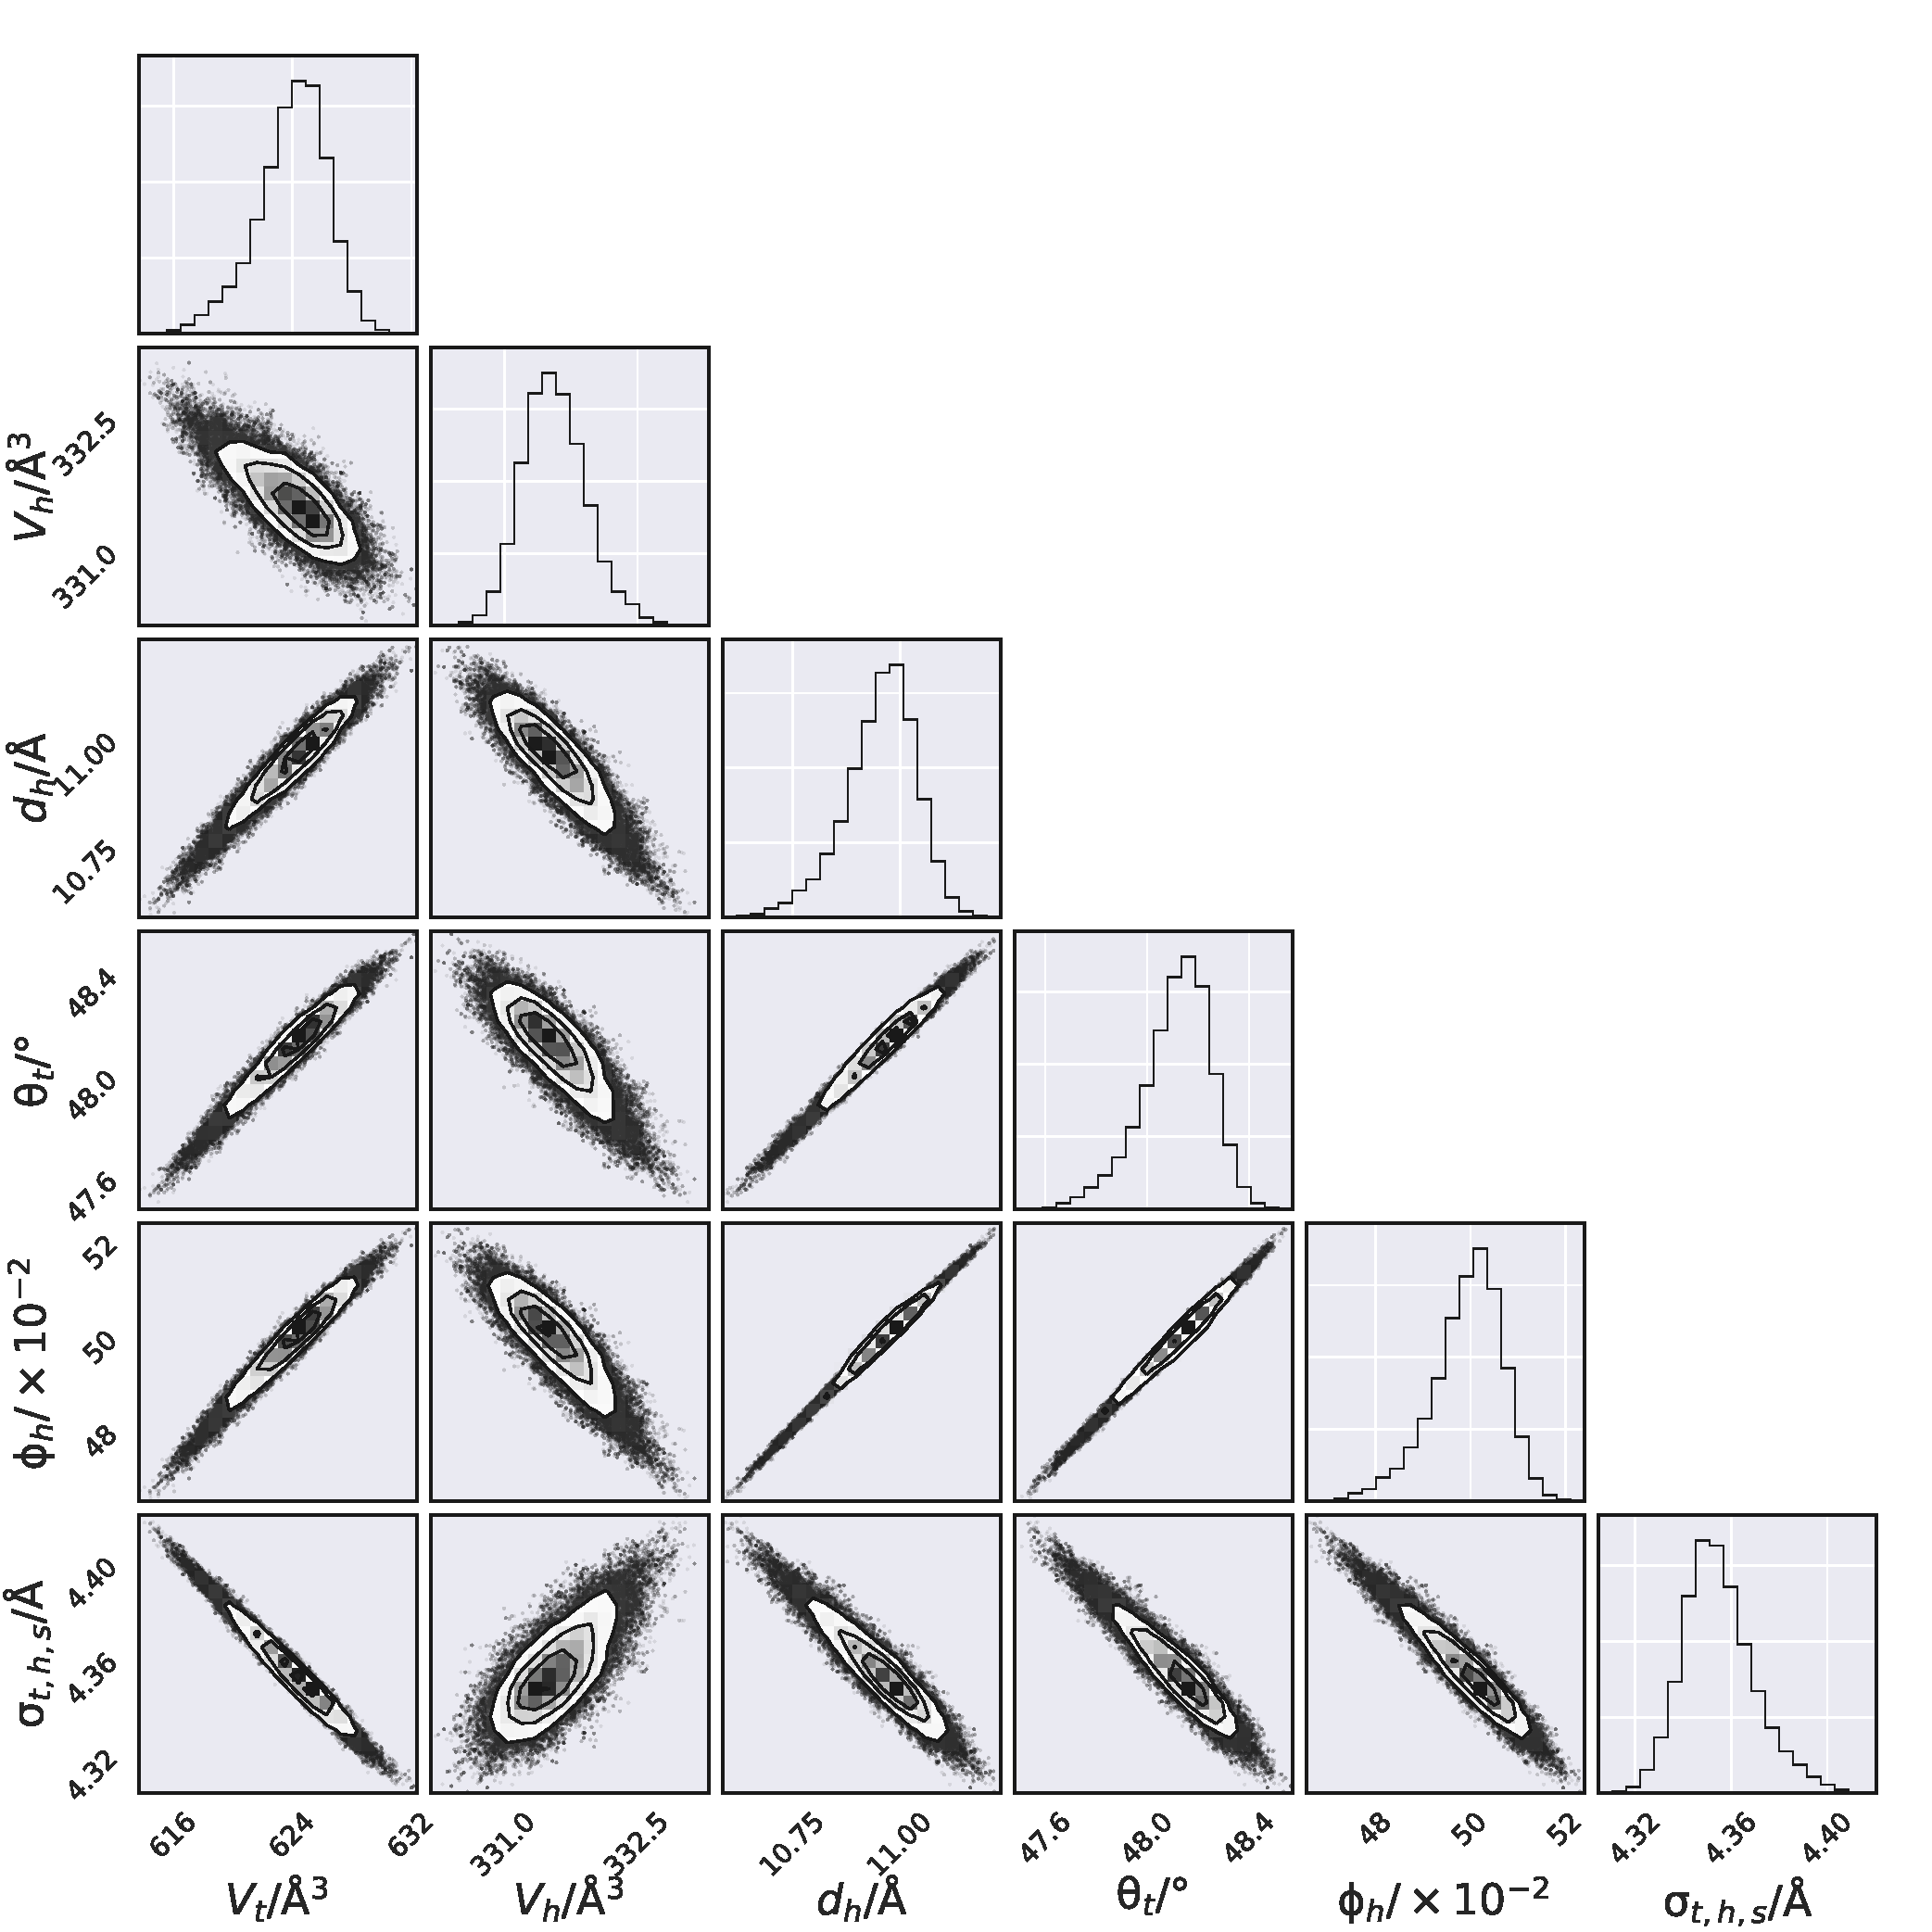
\includegraphics[width=0.50\textwidth]{figures/dlpc5_all_corner}
	\caption{The multi-parameter PDFs for the chemically-relevant model of DLPC X-ray reflectometry data at 35 mNm$^{-1}$. Source: Datasets, figure files and running/plotting scripts are available under CC-BY.\cite{mccluskey_2018}}
	\label{fig:dlpc5}
\end{figure}
\begin{figure}[h]
	\centering
	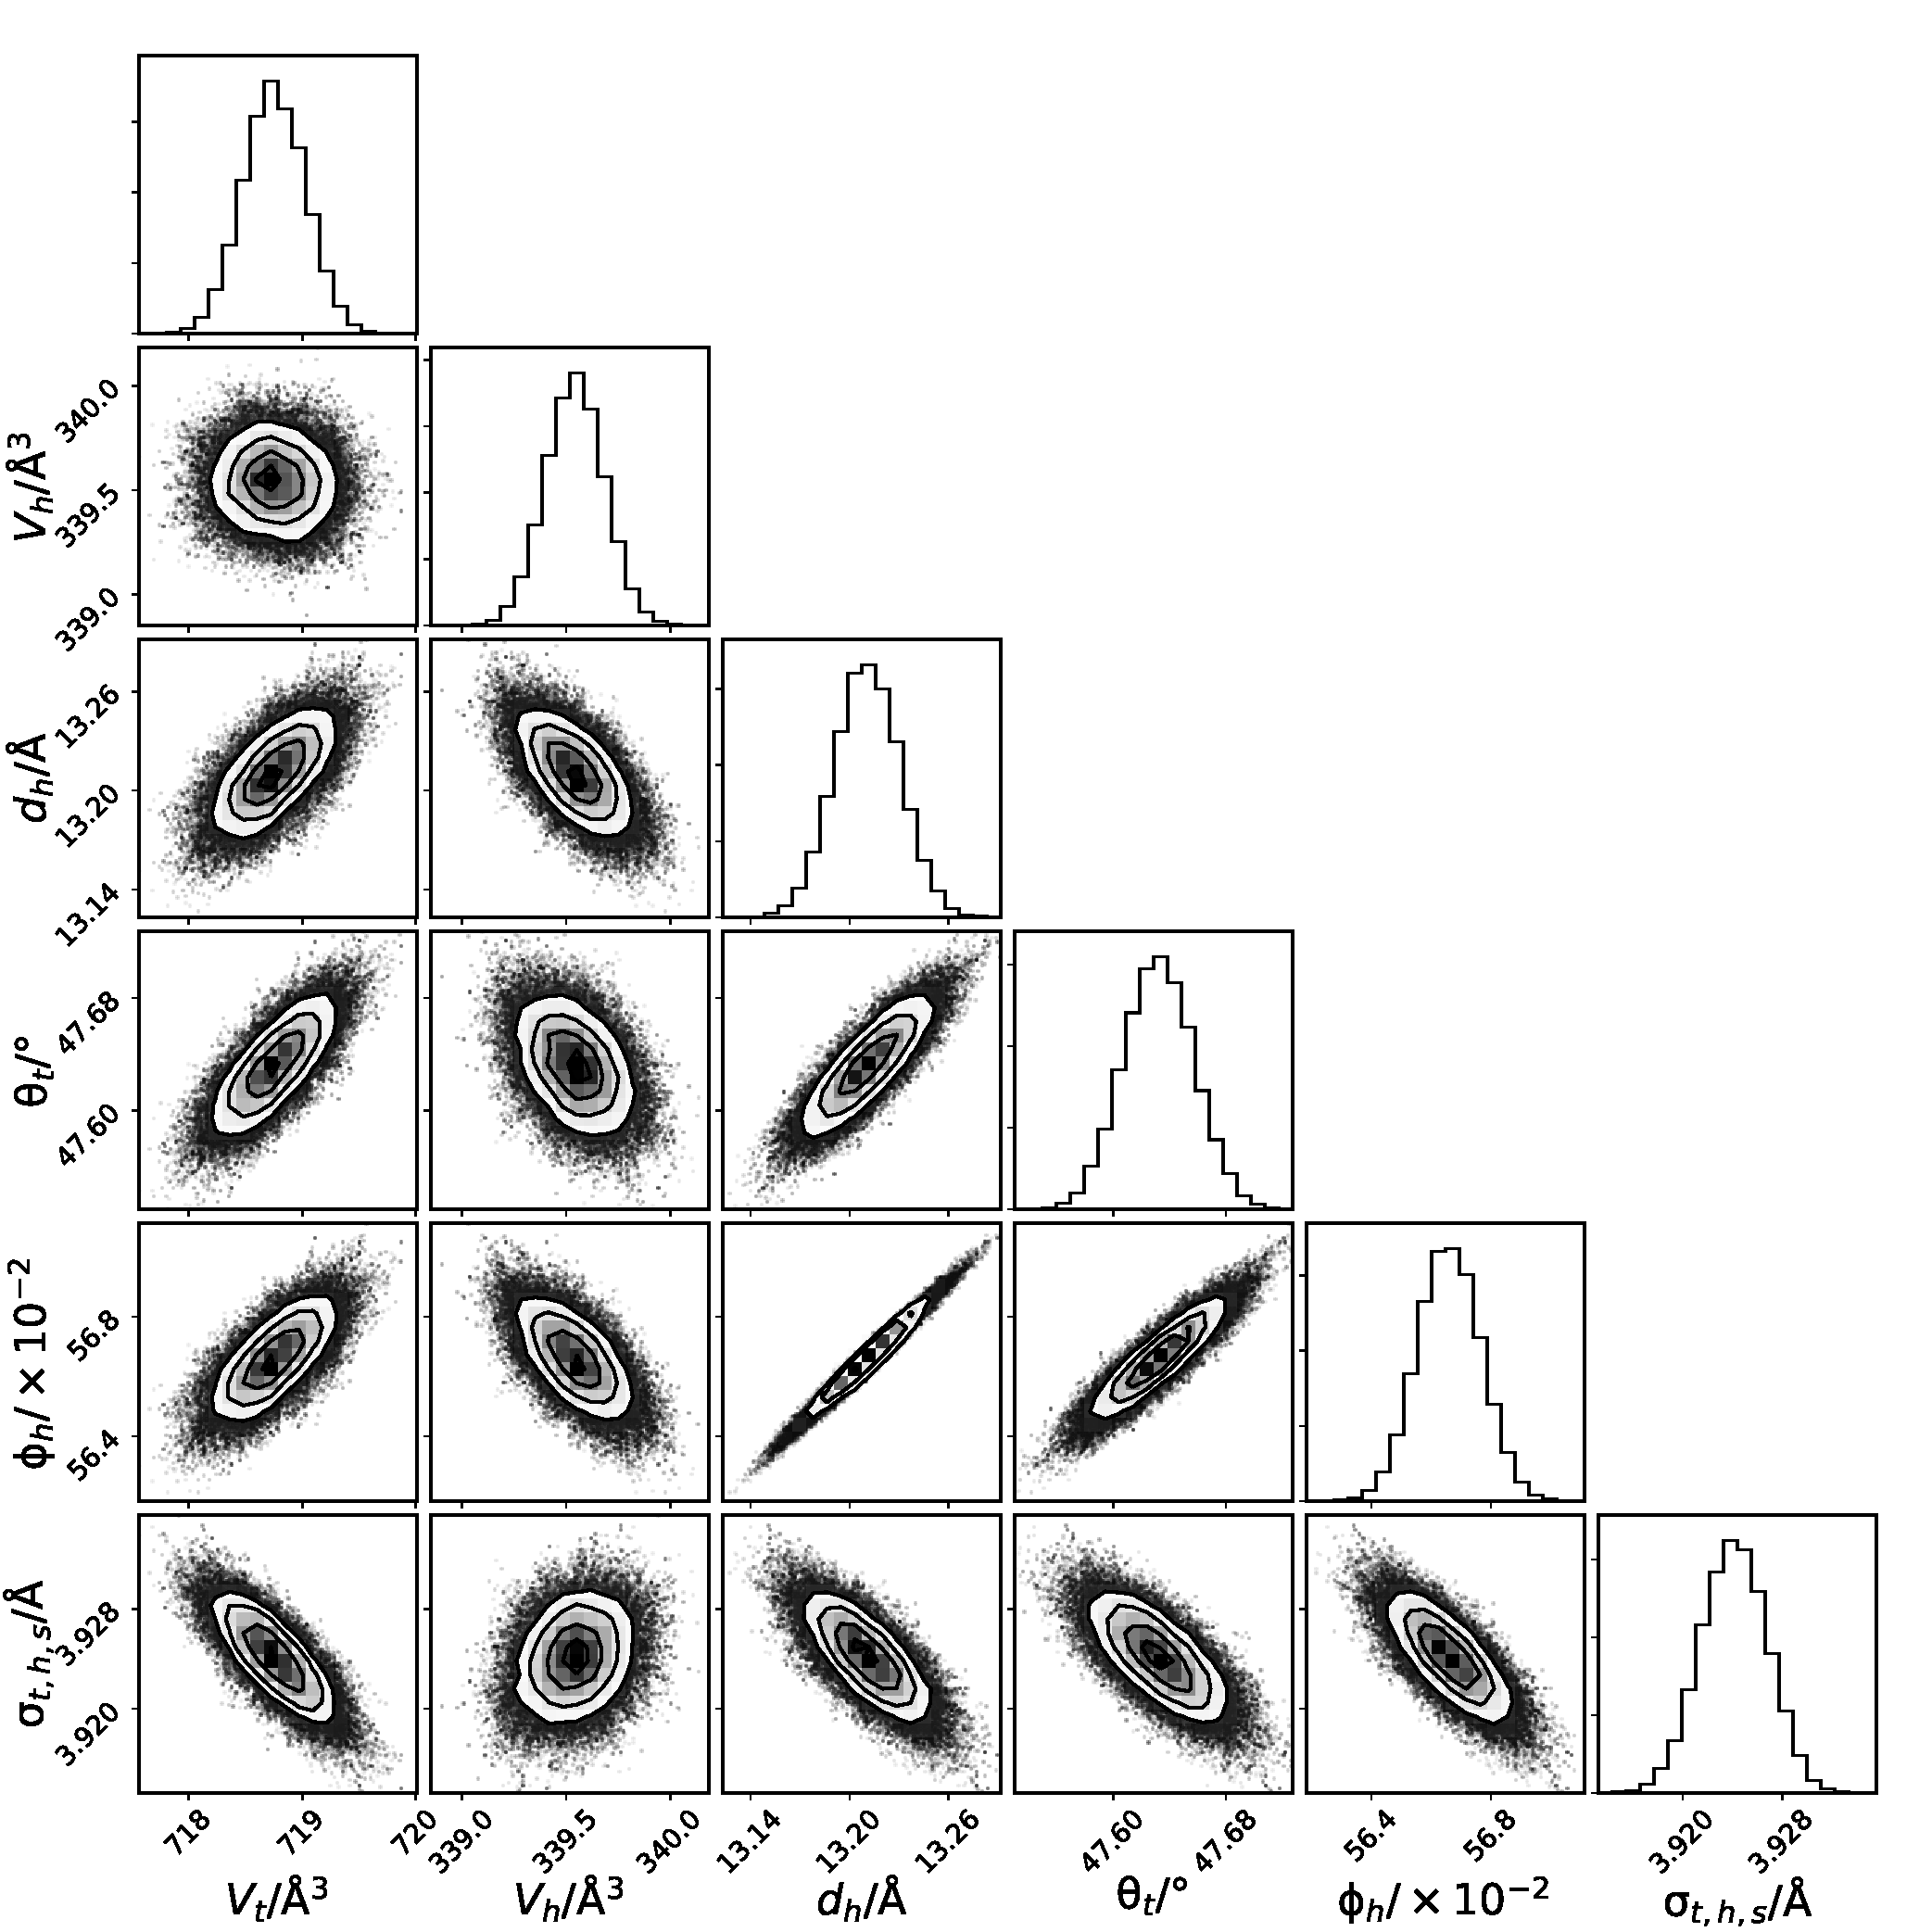
\includegraphics[width=0.50\textwidth]{figures/dmpc2_all_corner}
	\caption{The multi-parameter PDFs for the chemically-relevant model of DMPC X-ray reflectometry data at 20 mNm$^{-1}$. Source: Datasets, figure files and running/plotting scripts are available under CC-BY.\cite{mccluskey_2018}}
	\label{fig:dmpc2}
\end{figure}
\begin{figure}[h]
	\centering
	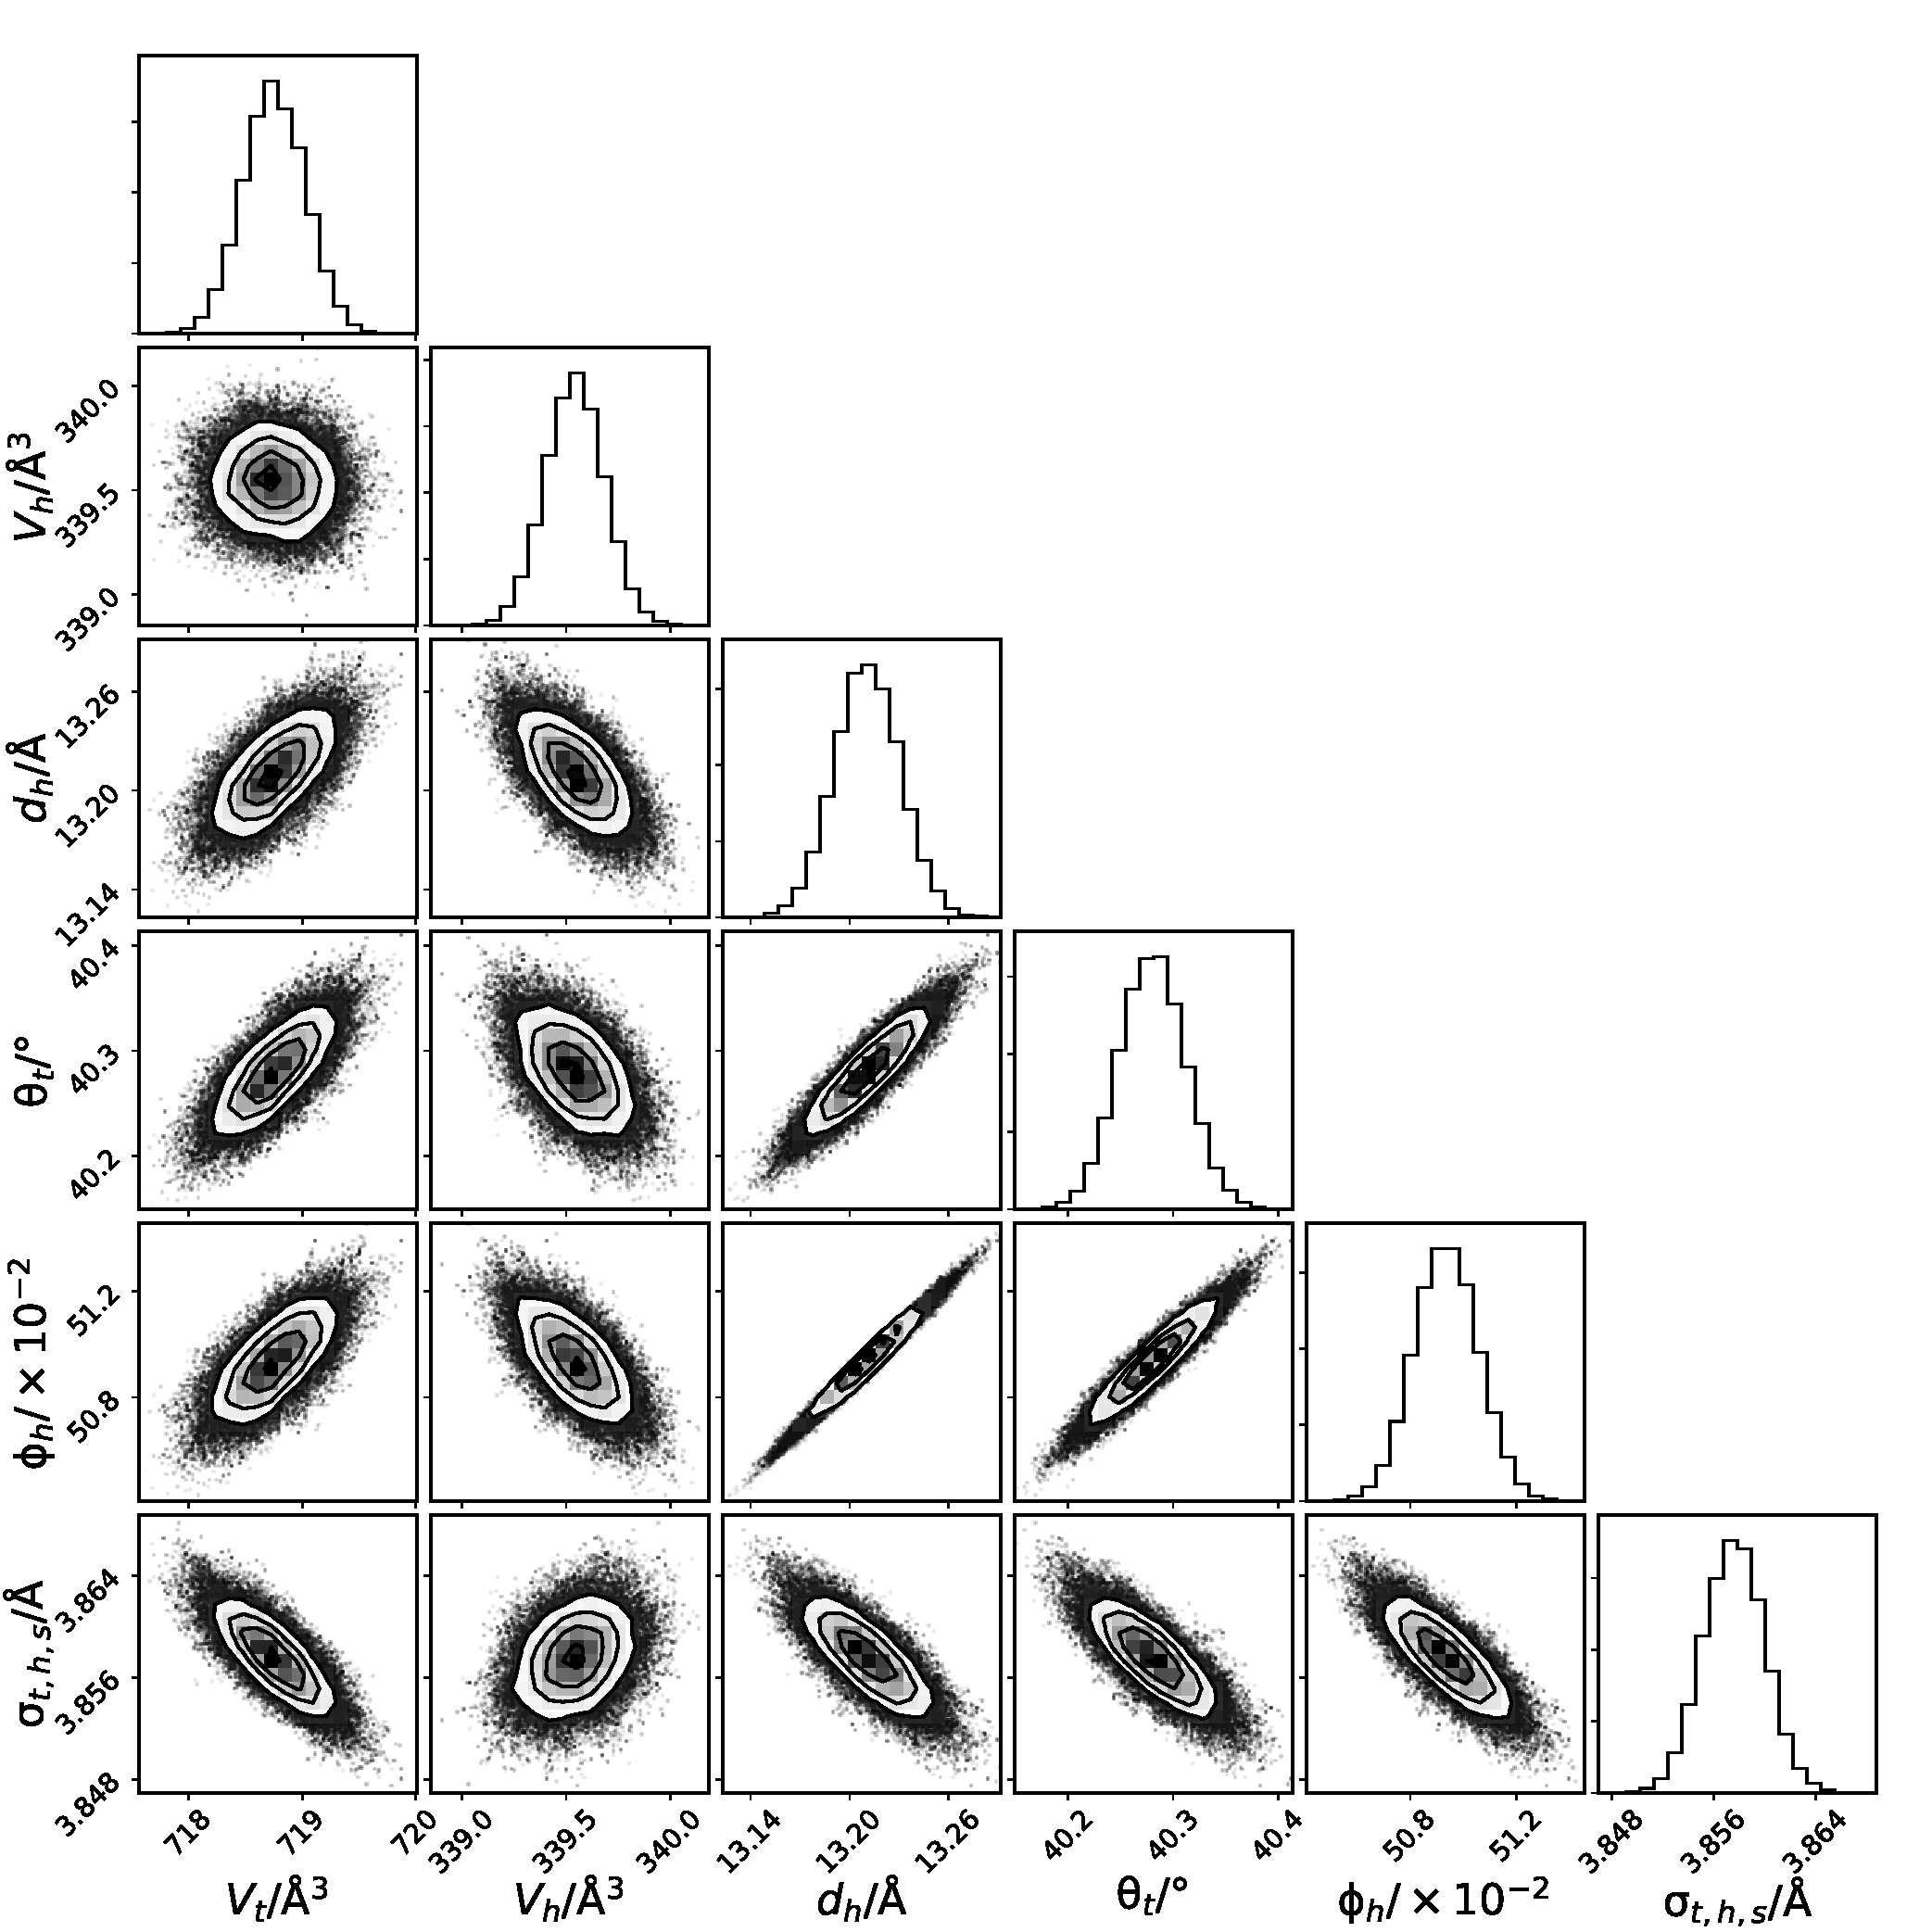
\includegraphics[width=0.50\textwidth]{figures/dmpc3_all_corner}
	\caption{The multi-parameter PDFs for the chemically-relevant model of DMPC X-ray reflectometry data at 25 mNm$^{-1}$. Source: Datasets, figure files and running/plotting scripts are available under CC-BY.\cite{mccluskey_2018}}
	\label{fig:dmpc3}
\end{figure}
\begin{figure}[h]
	\centering
	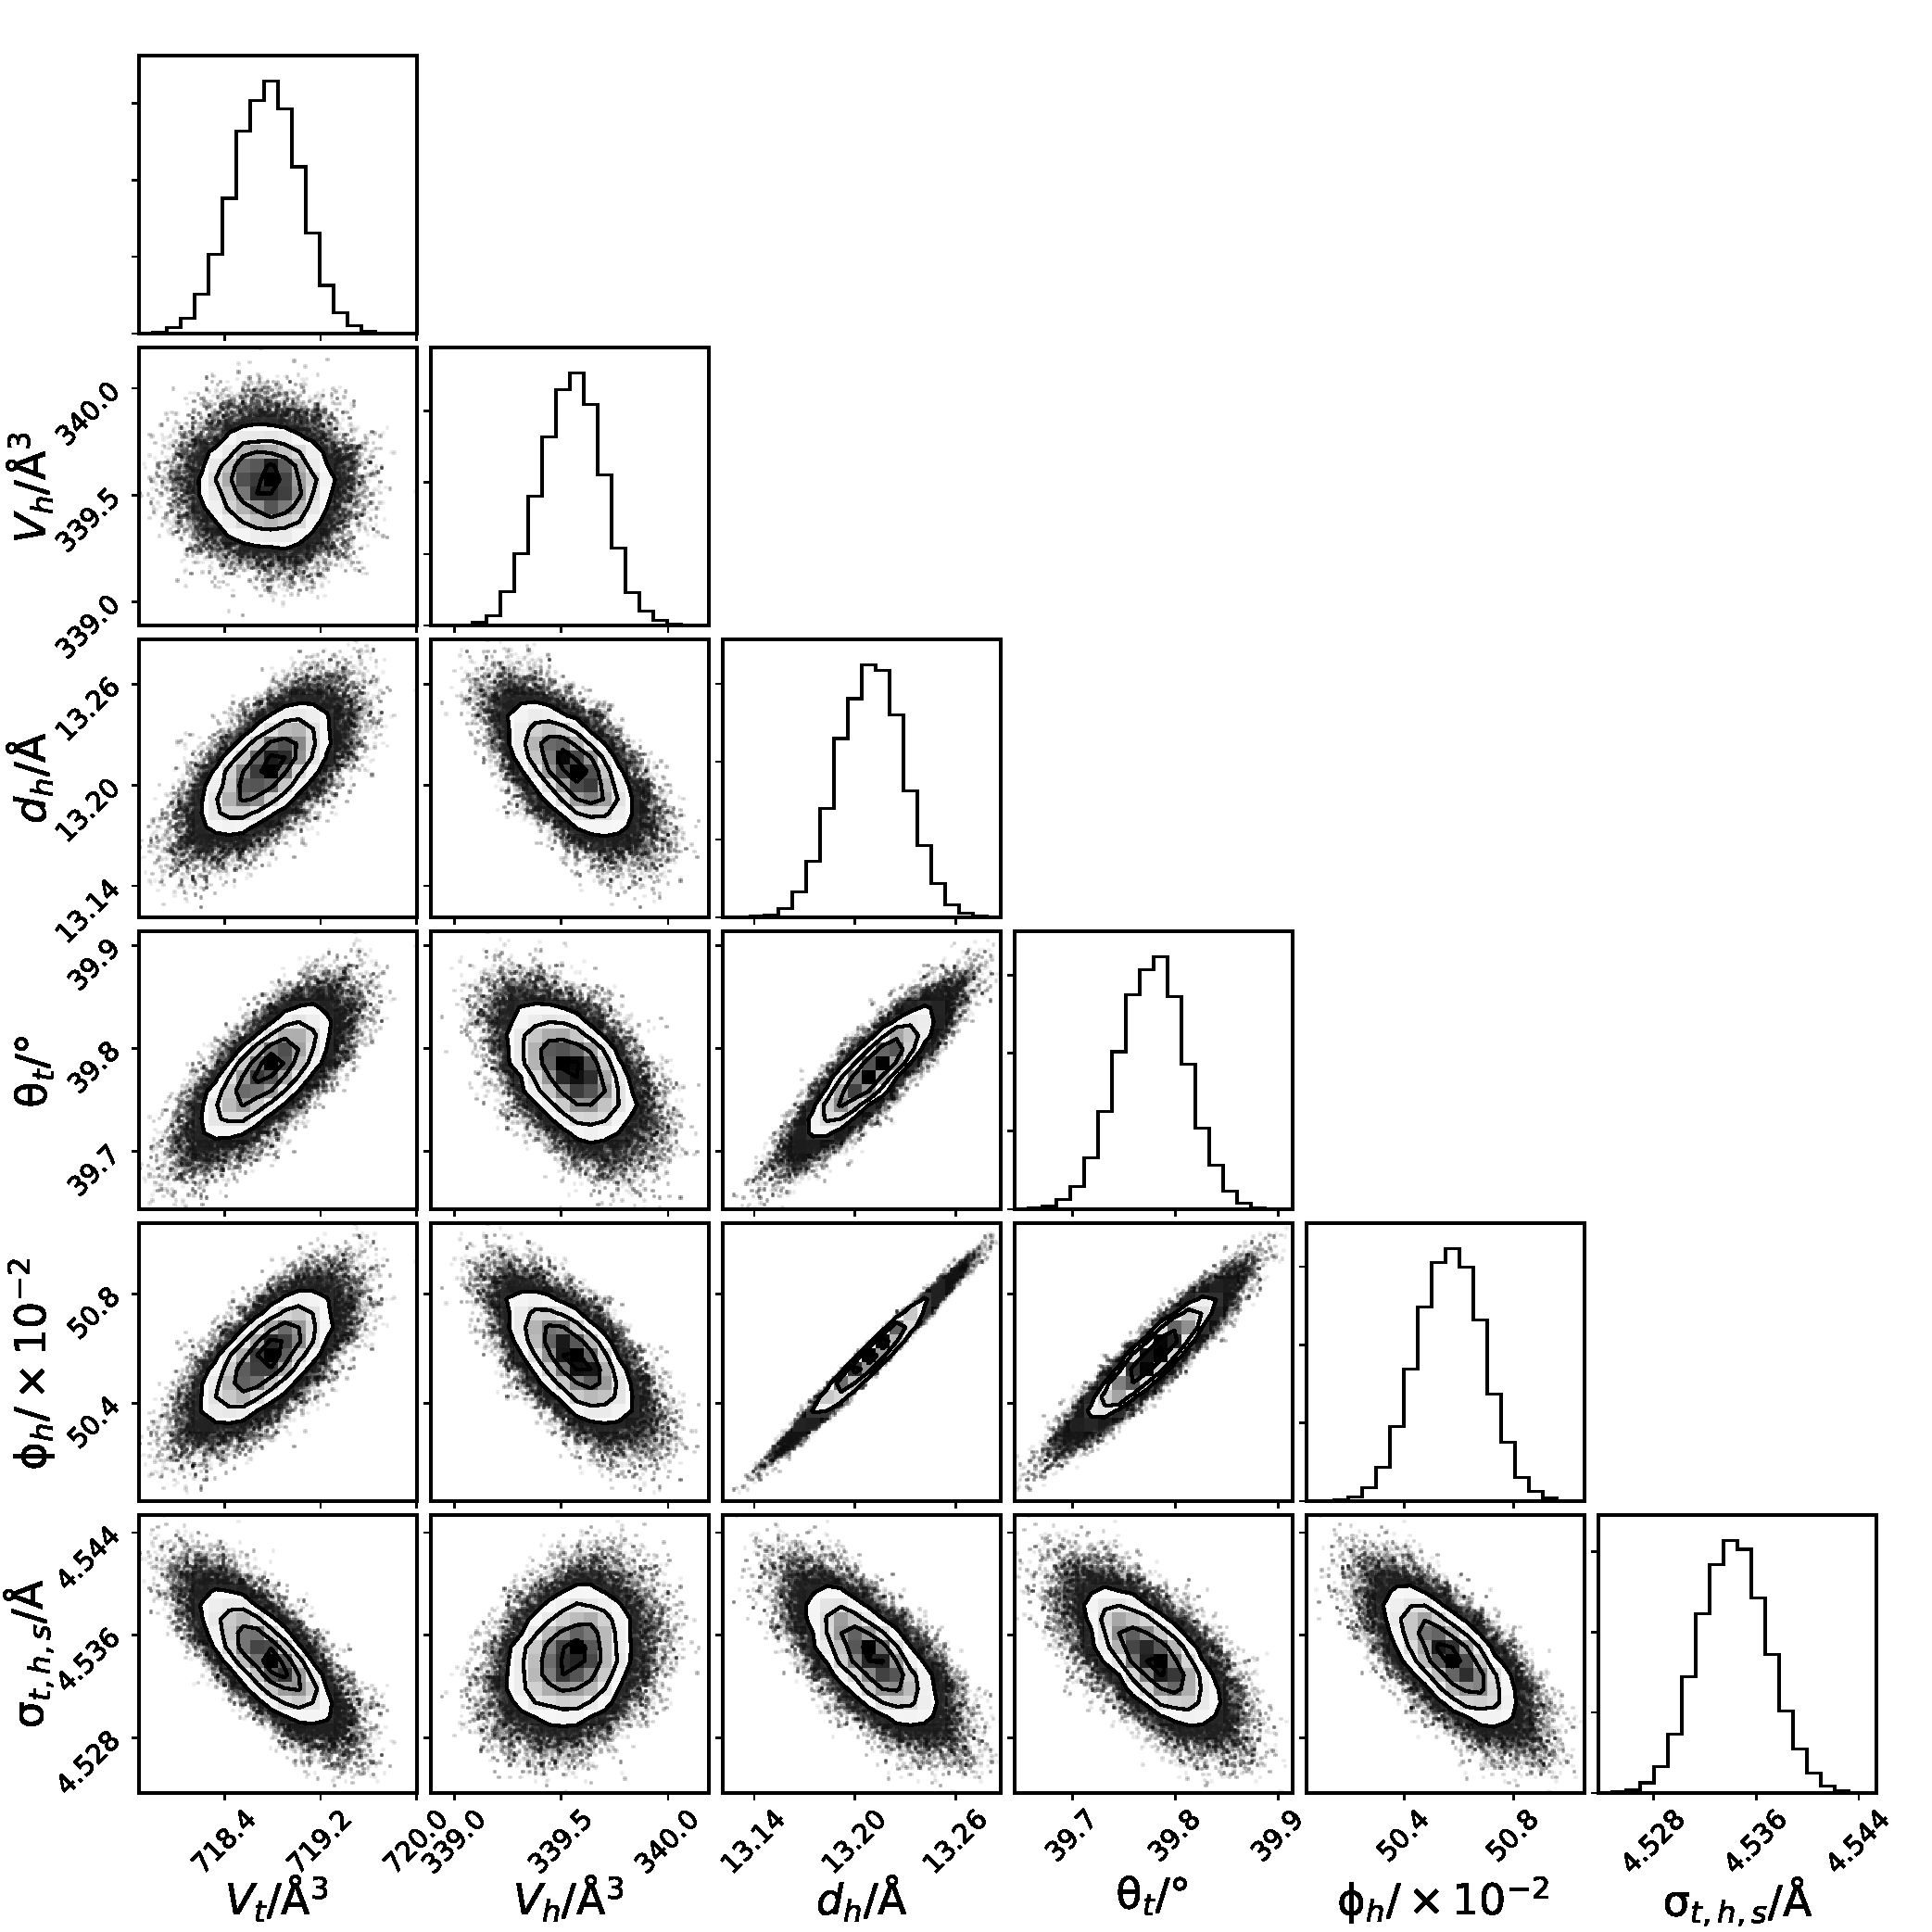
\includegraphics[width=0.50\textwidth]{figures/dmpc4_all_corner}
	\caption{The multi-parameter PDFs for the chemically-relevant model of DMPC X-ray reflectometry data at 30 mNm$^{-1}$. Source: Datasets, figure files and running/plotting scripts are available under CC-BY.\cite{mccluskey_2018}}
	\label{fig:dmpc4}
\end{figure}
\begin{figure}
	\centering
	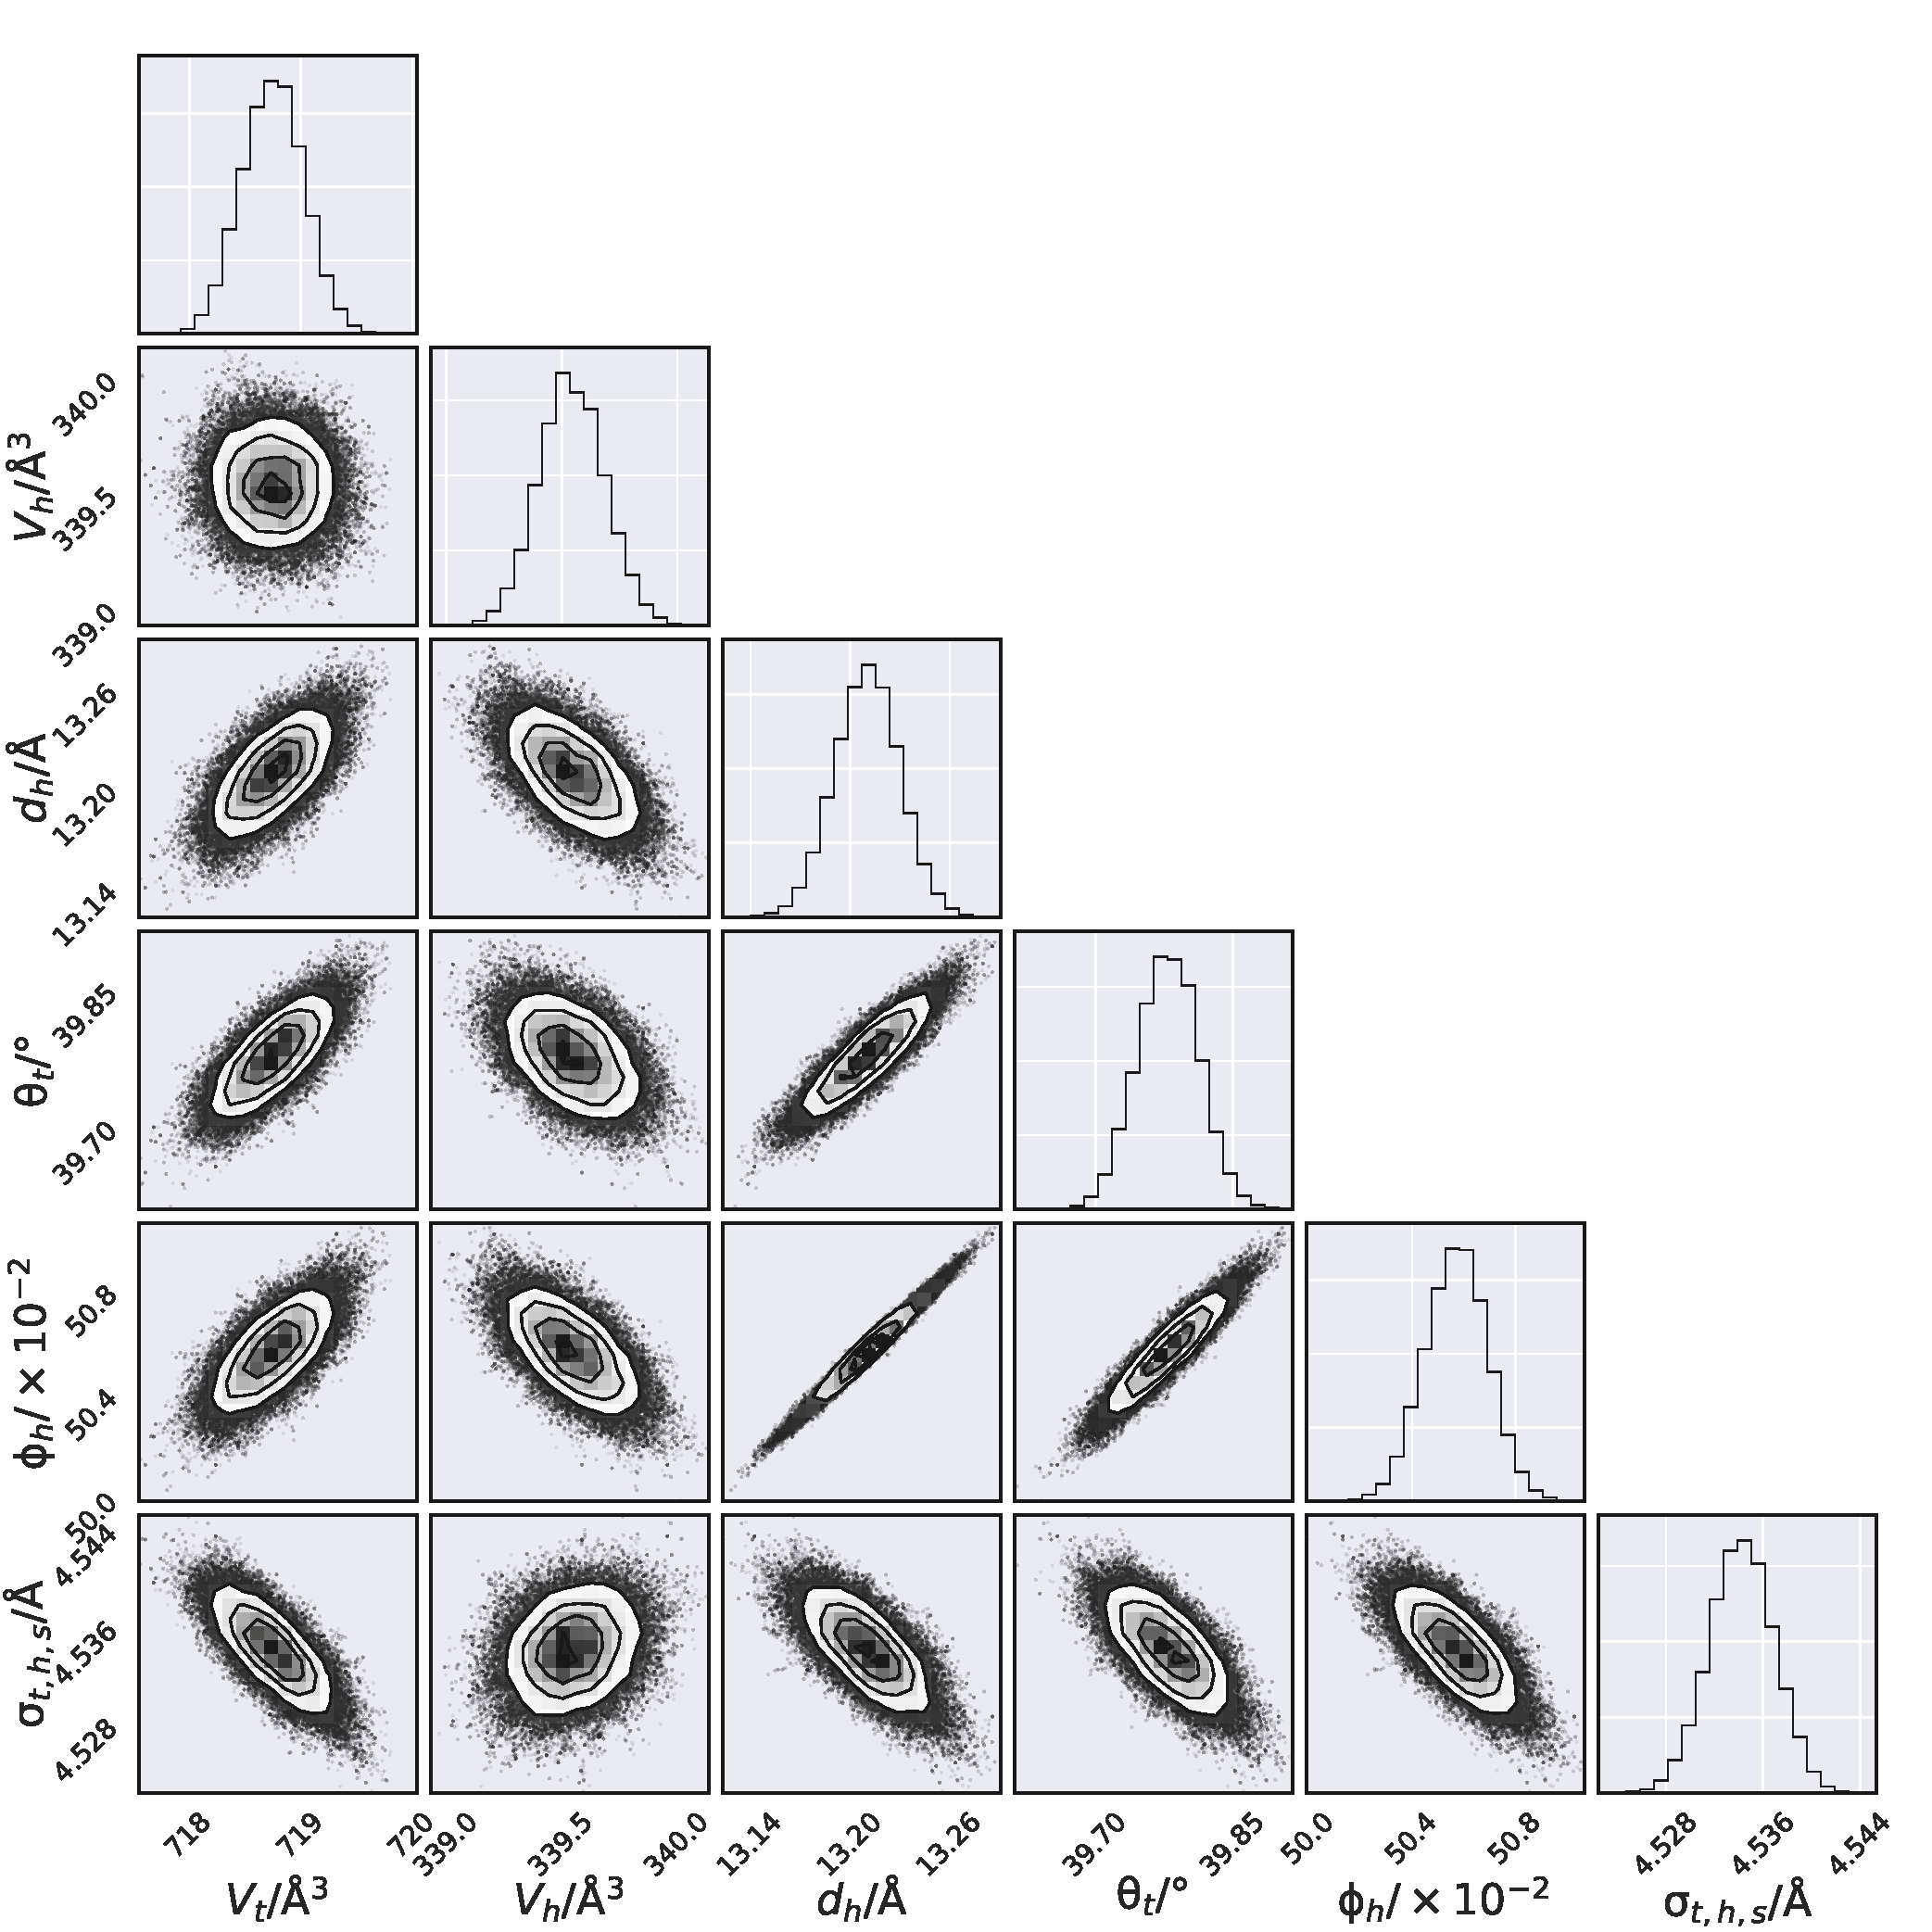
\includegraphics[width=0.50\textwidth]{figures/dmpc5_all_corner}
	\caption{The multi-parameter PDFs for the chemically-relevant model of DMPC X-ray reflectometry data at 40 mNm$^{-1}$. Source: Datasets, figure files and running/plotting scripts are available under CC-BY.\cite{mccluskey_2018}}
	\label{fig:dmpc5}
\end{figure}
\begin{figure}[h]
	\centering
	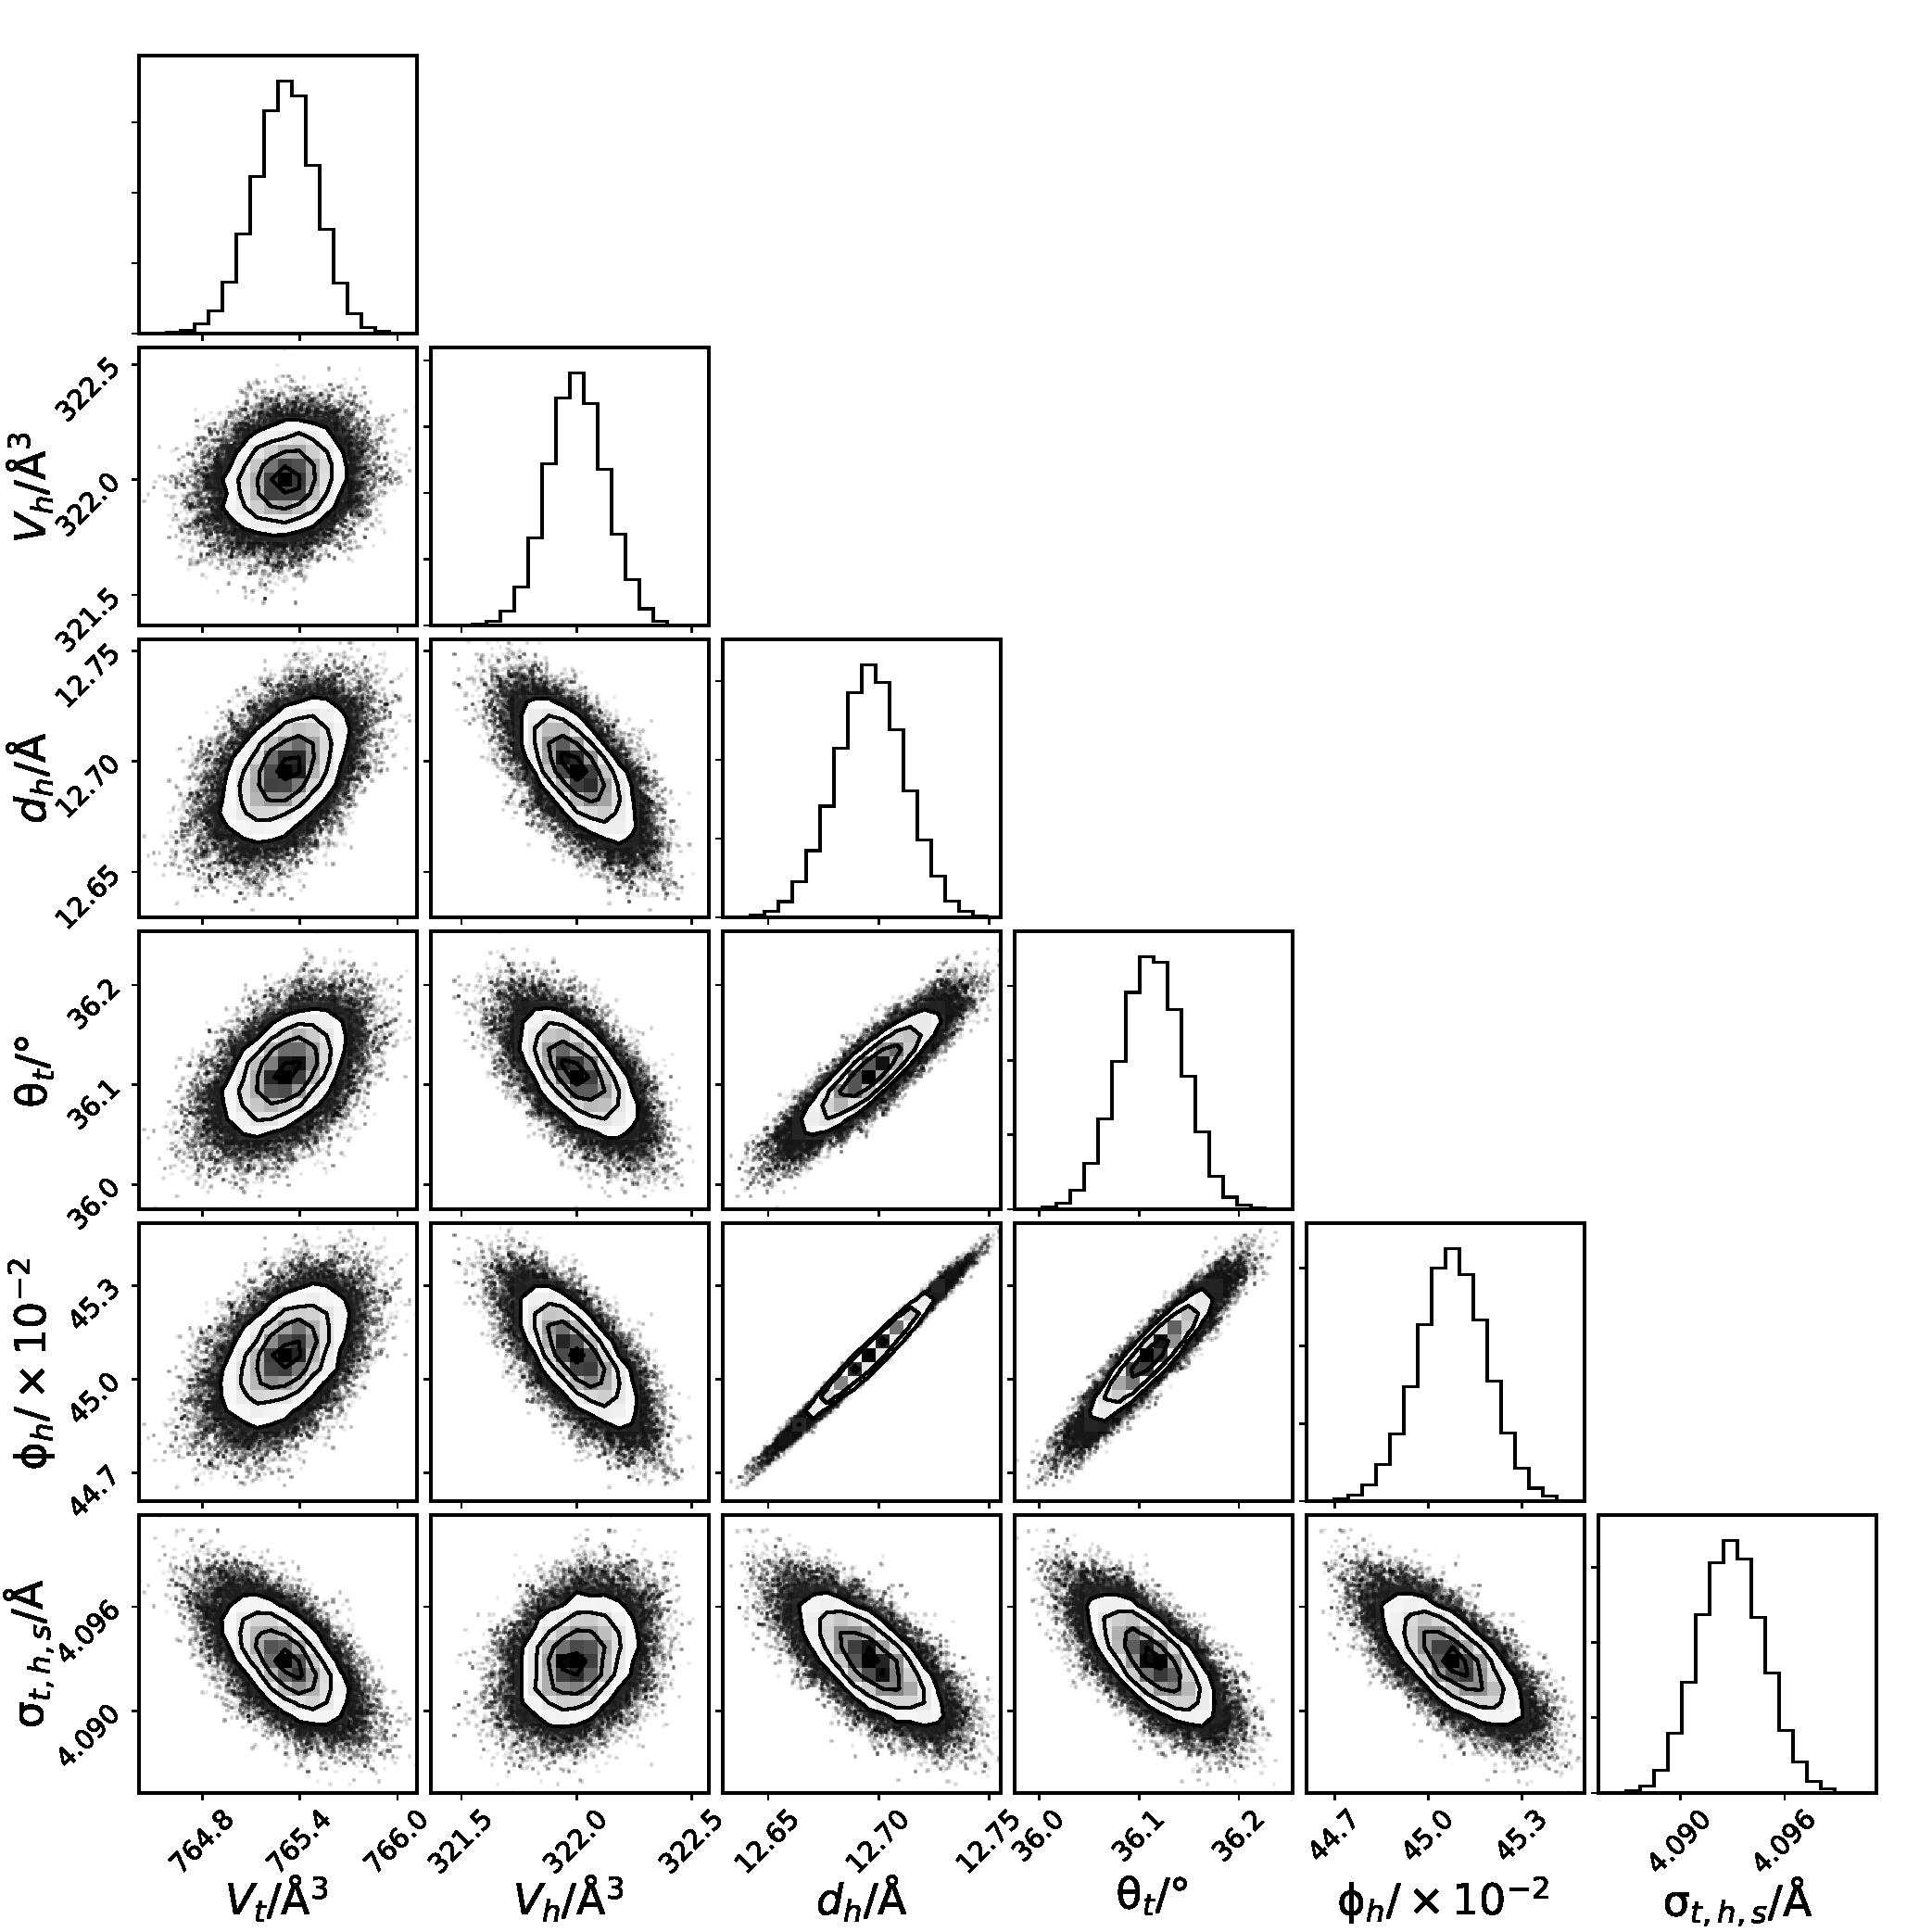
\includegraphics[width=0.50\textwidth]{figures/dppc2_all_corner}
	\caption{The multi-parameter PDFs for the chemically-relevant model of DPPC X-ray reflectometry data at 15 mNm$^{-1}$. Source: Datasets, figure files and running/plotting scripts are available under CC-BY.\cite{mccluskey_2018}}
	\label{fig:dppc2}
\end{figure}
\begin{figure}[h]
	\centering
	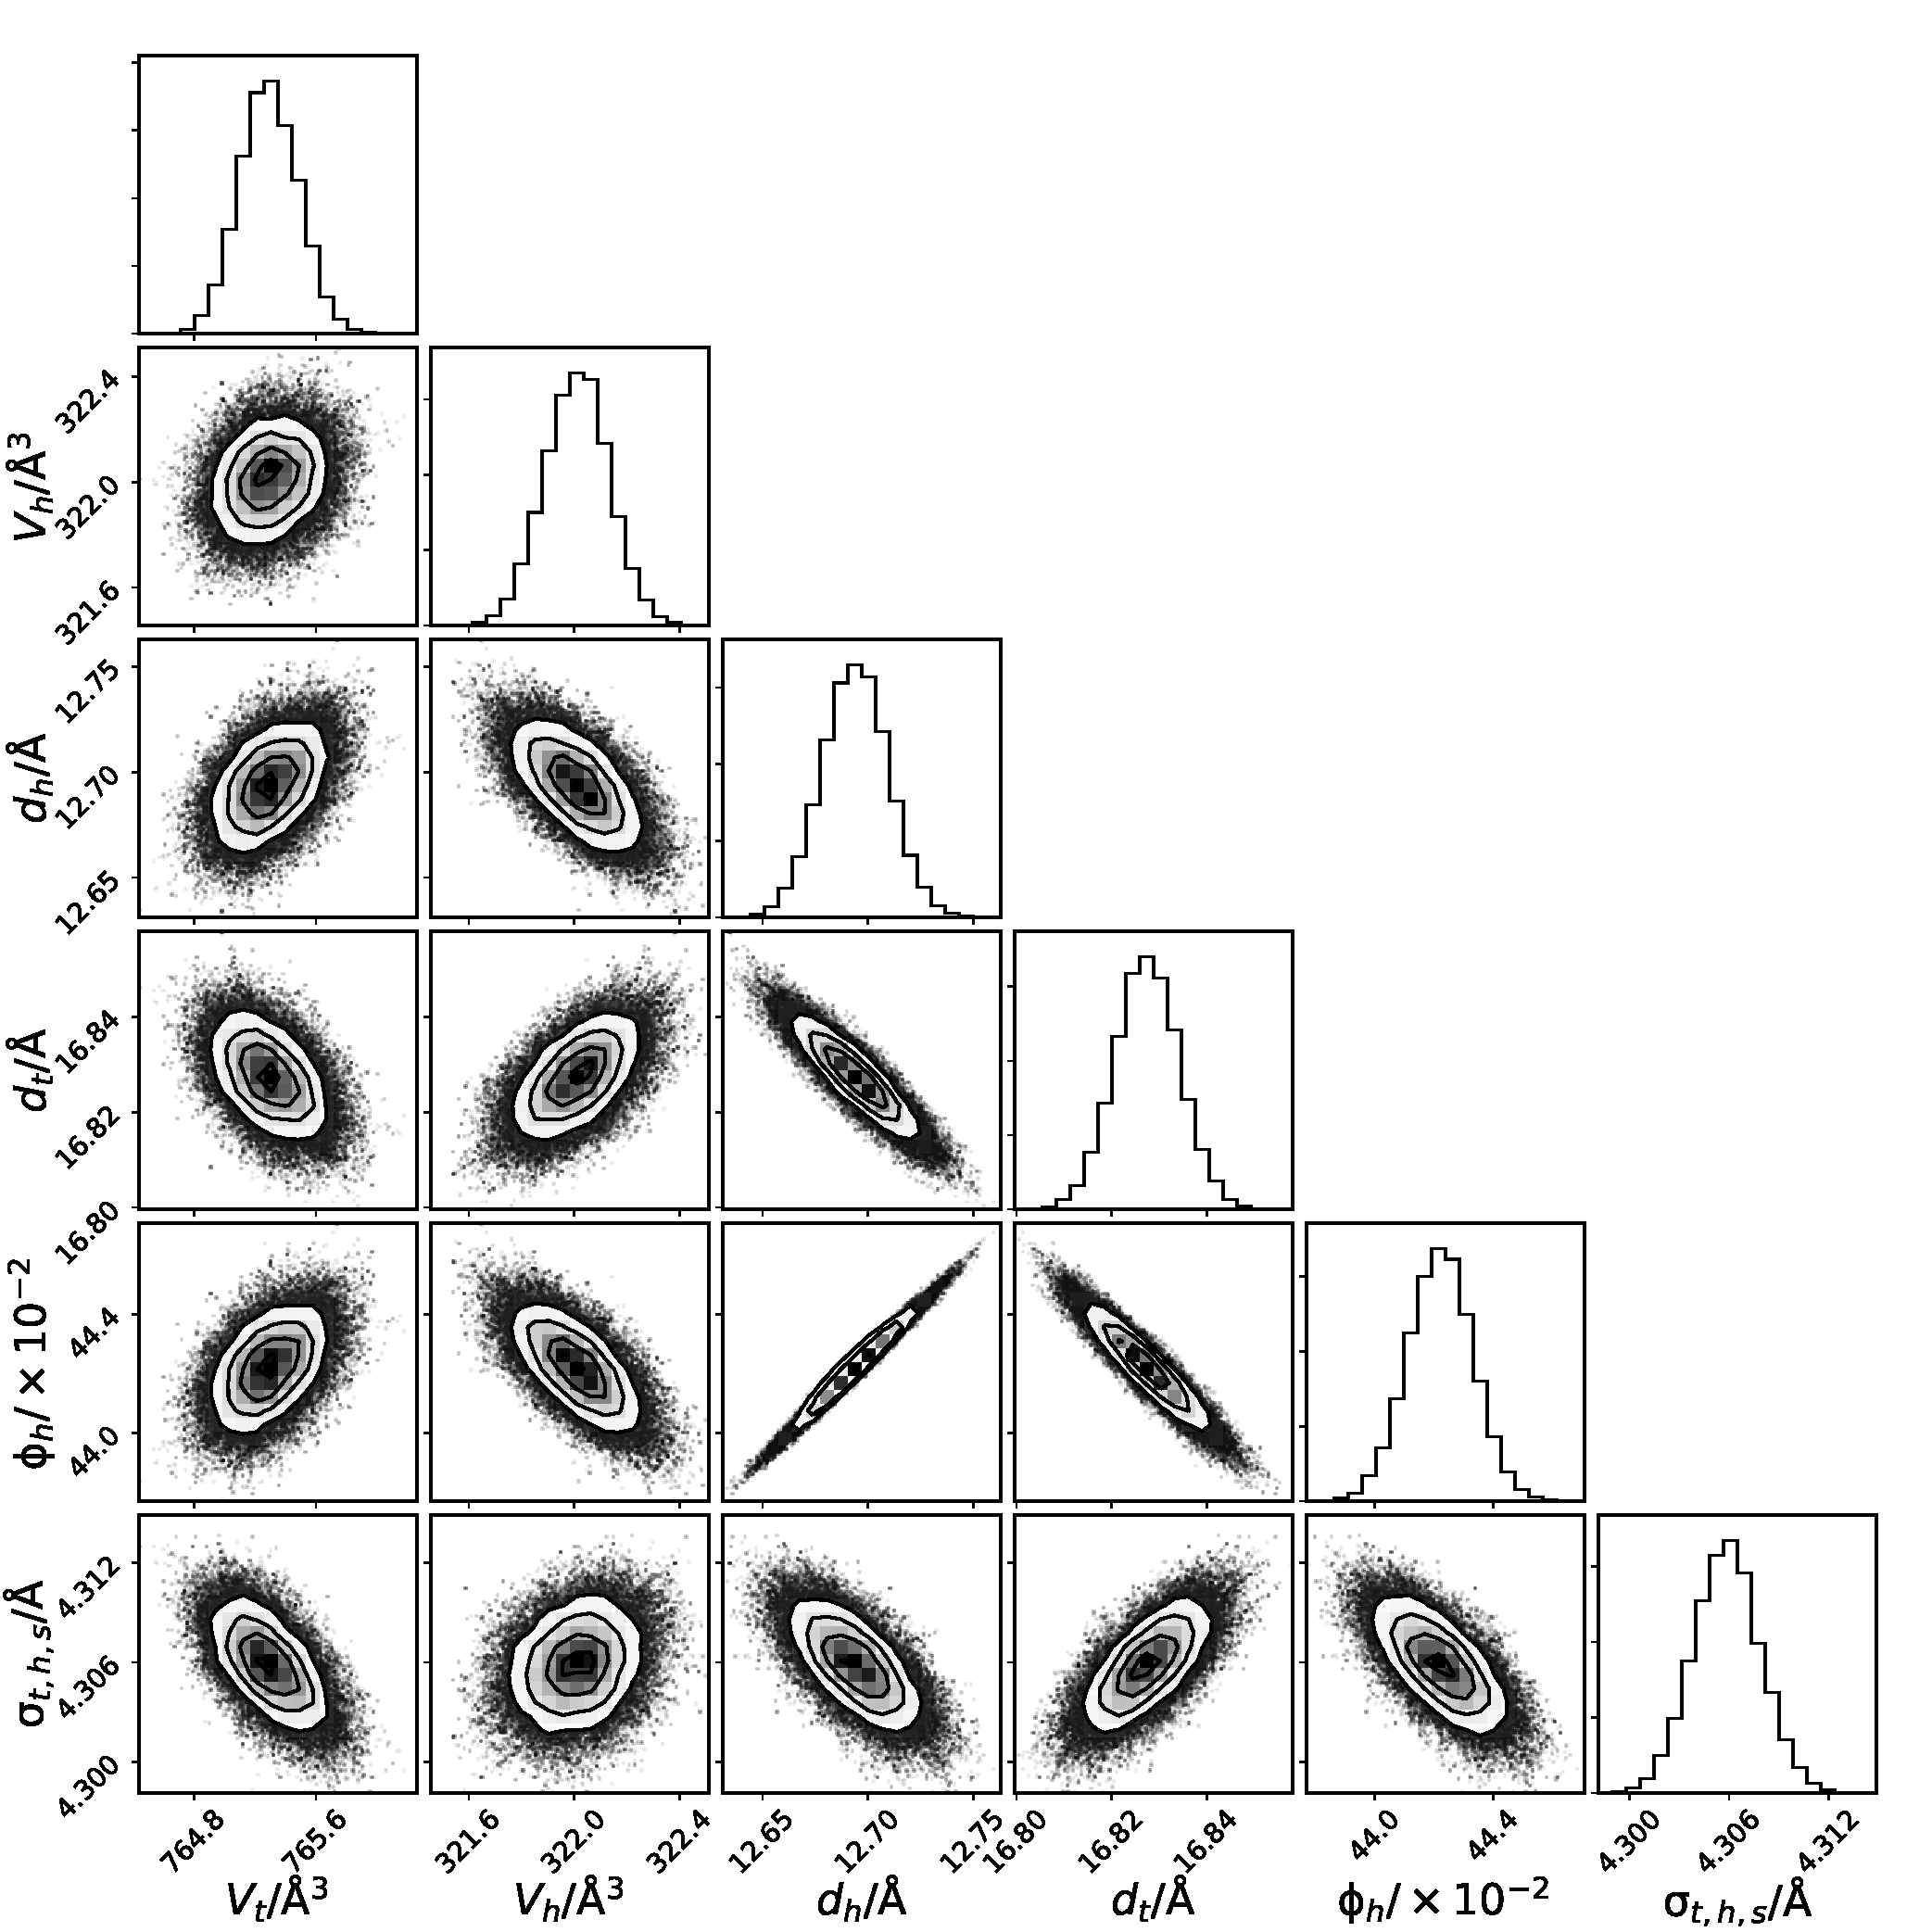
\includegraphics[width=0.50\textwidth]{figures/dppc3_all_corner}
	\caption{The multi-parameter PDFs for the chemically-relevant model of DPPC X-ray reflectometry data at 20 mNm$^{-1}$. Source: Datasets, figure files and running/plotting scripts are available under CC-BY.\cite{mccluskey_2018}}
	\label{fig:dppc3}
\end{figure}
\begin{figure}[h]
	\centering
	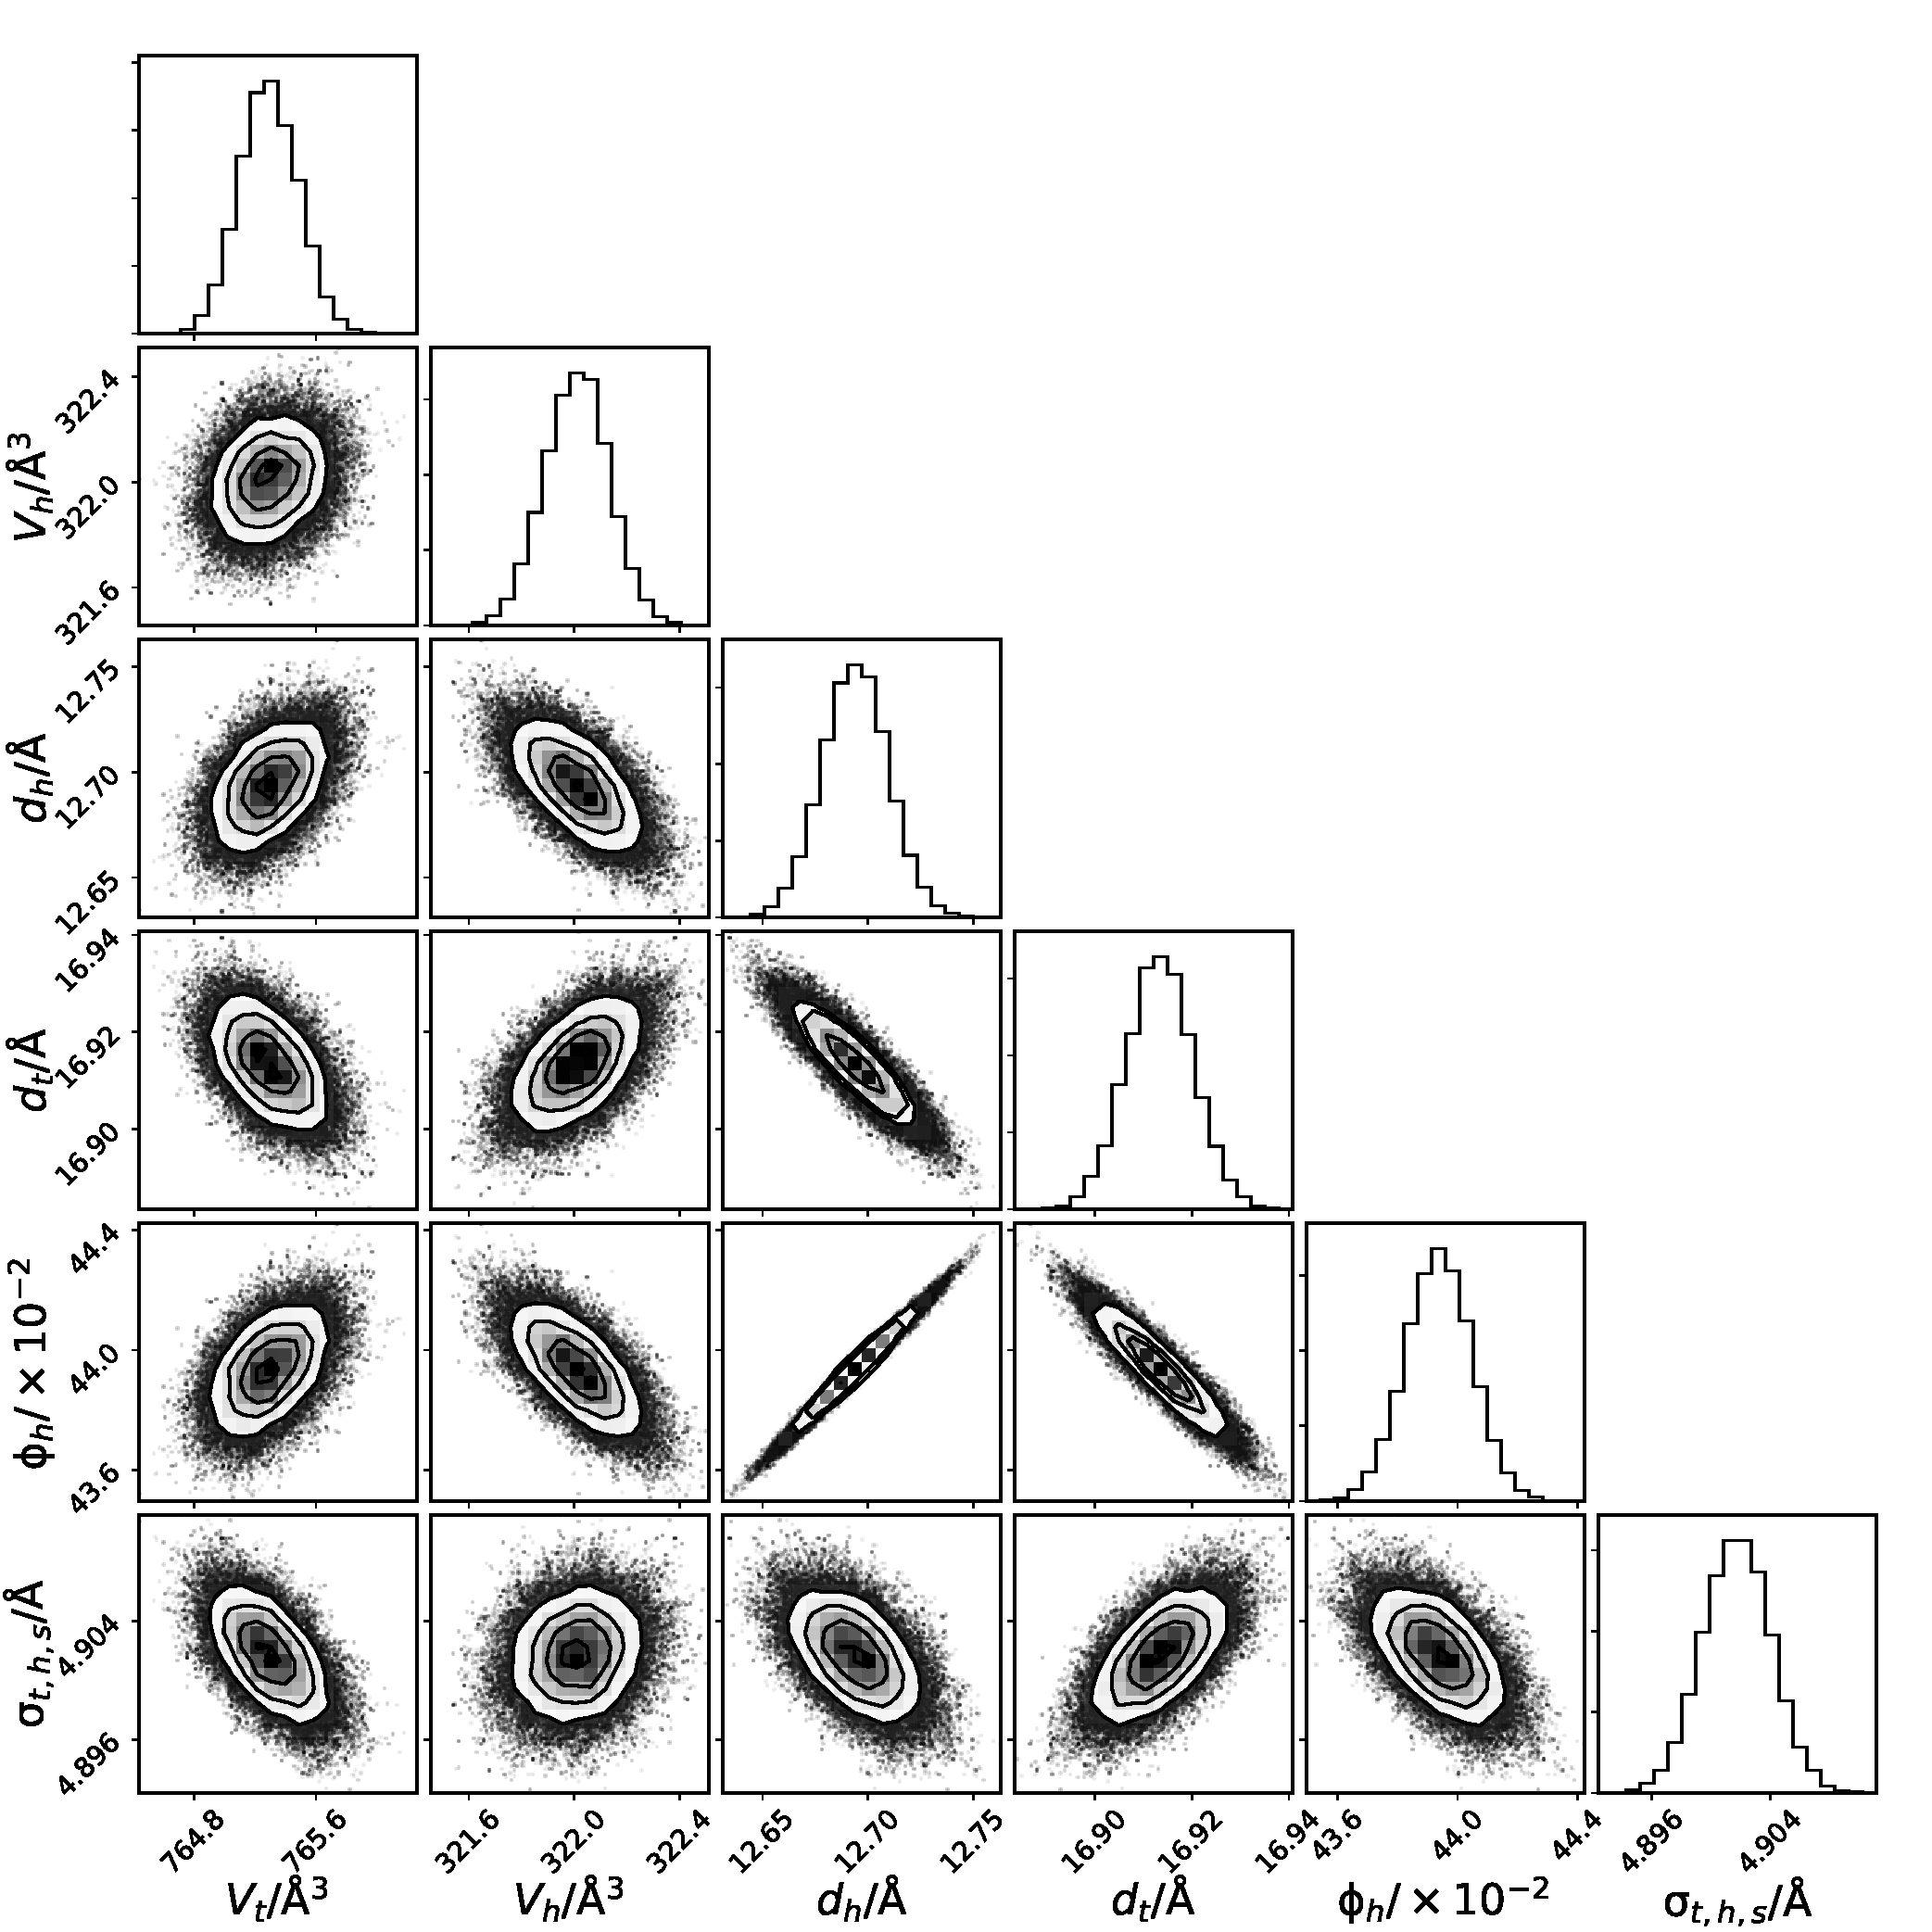
\includegraphics[width=0.50\textwidth]{figures/dppc4_all_corner}
	\caption{The multi-parameter PDFs for the chemically-relevant model of DPPC X-ray reflectometry data at 25 mNm$^{-1}$. Source: Datasets, figure files and running/plotting scripts are available under CC-BY.\cite{mccluskey_2018}}
	\label{fig:dppc4}
\end{figure}
\begin{figure}
	\centering
	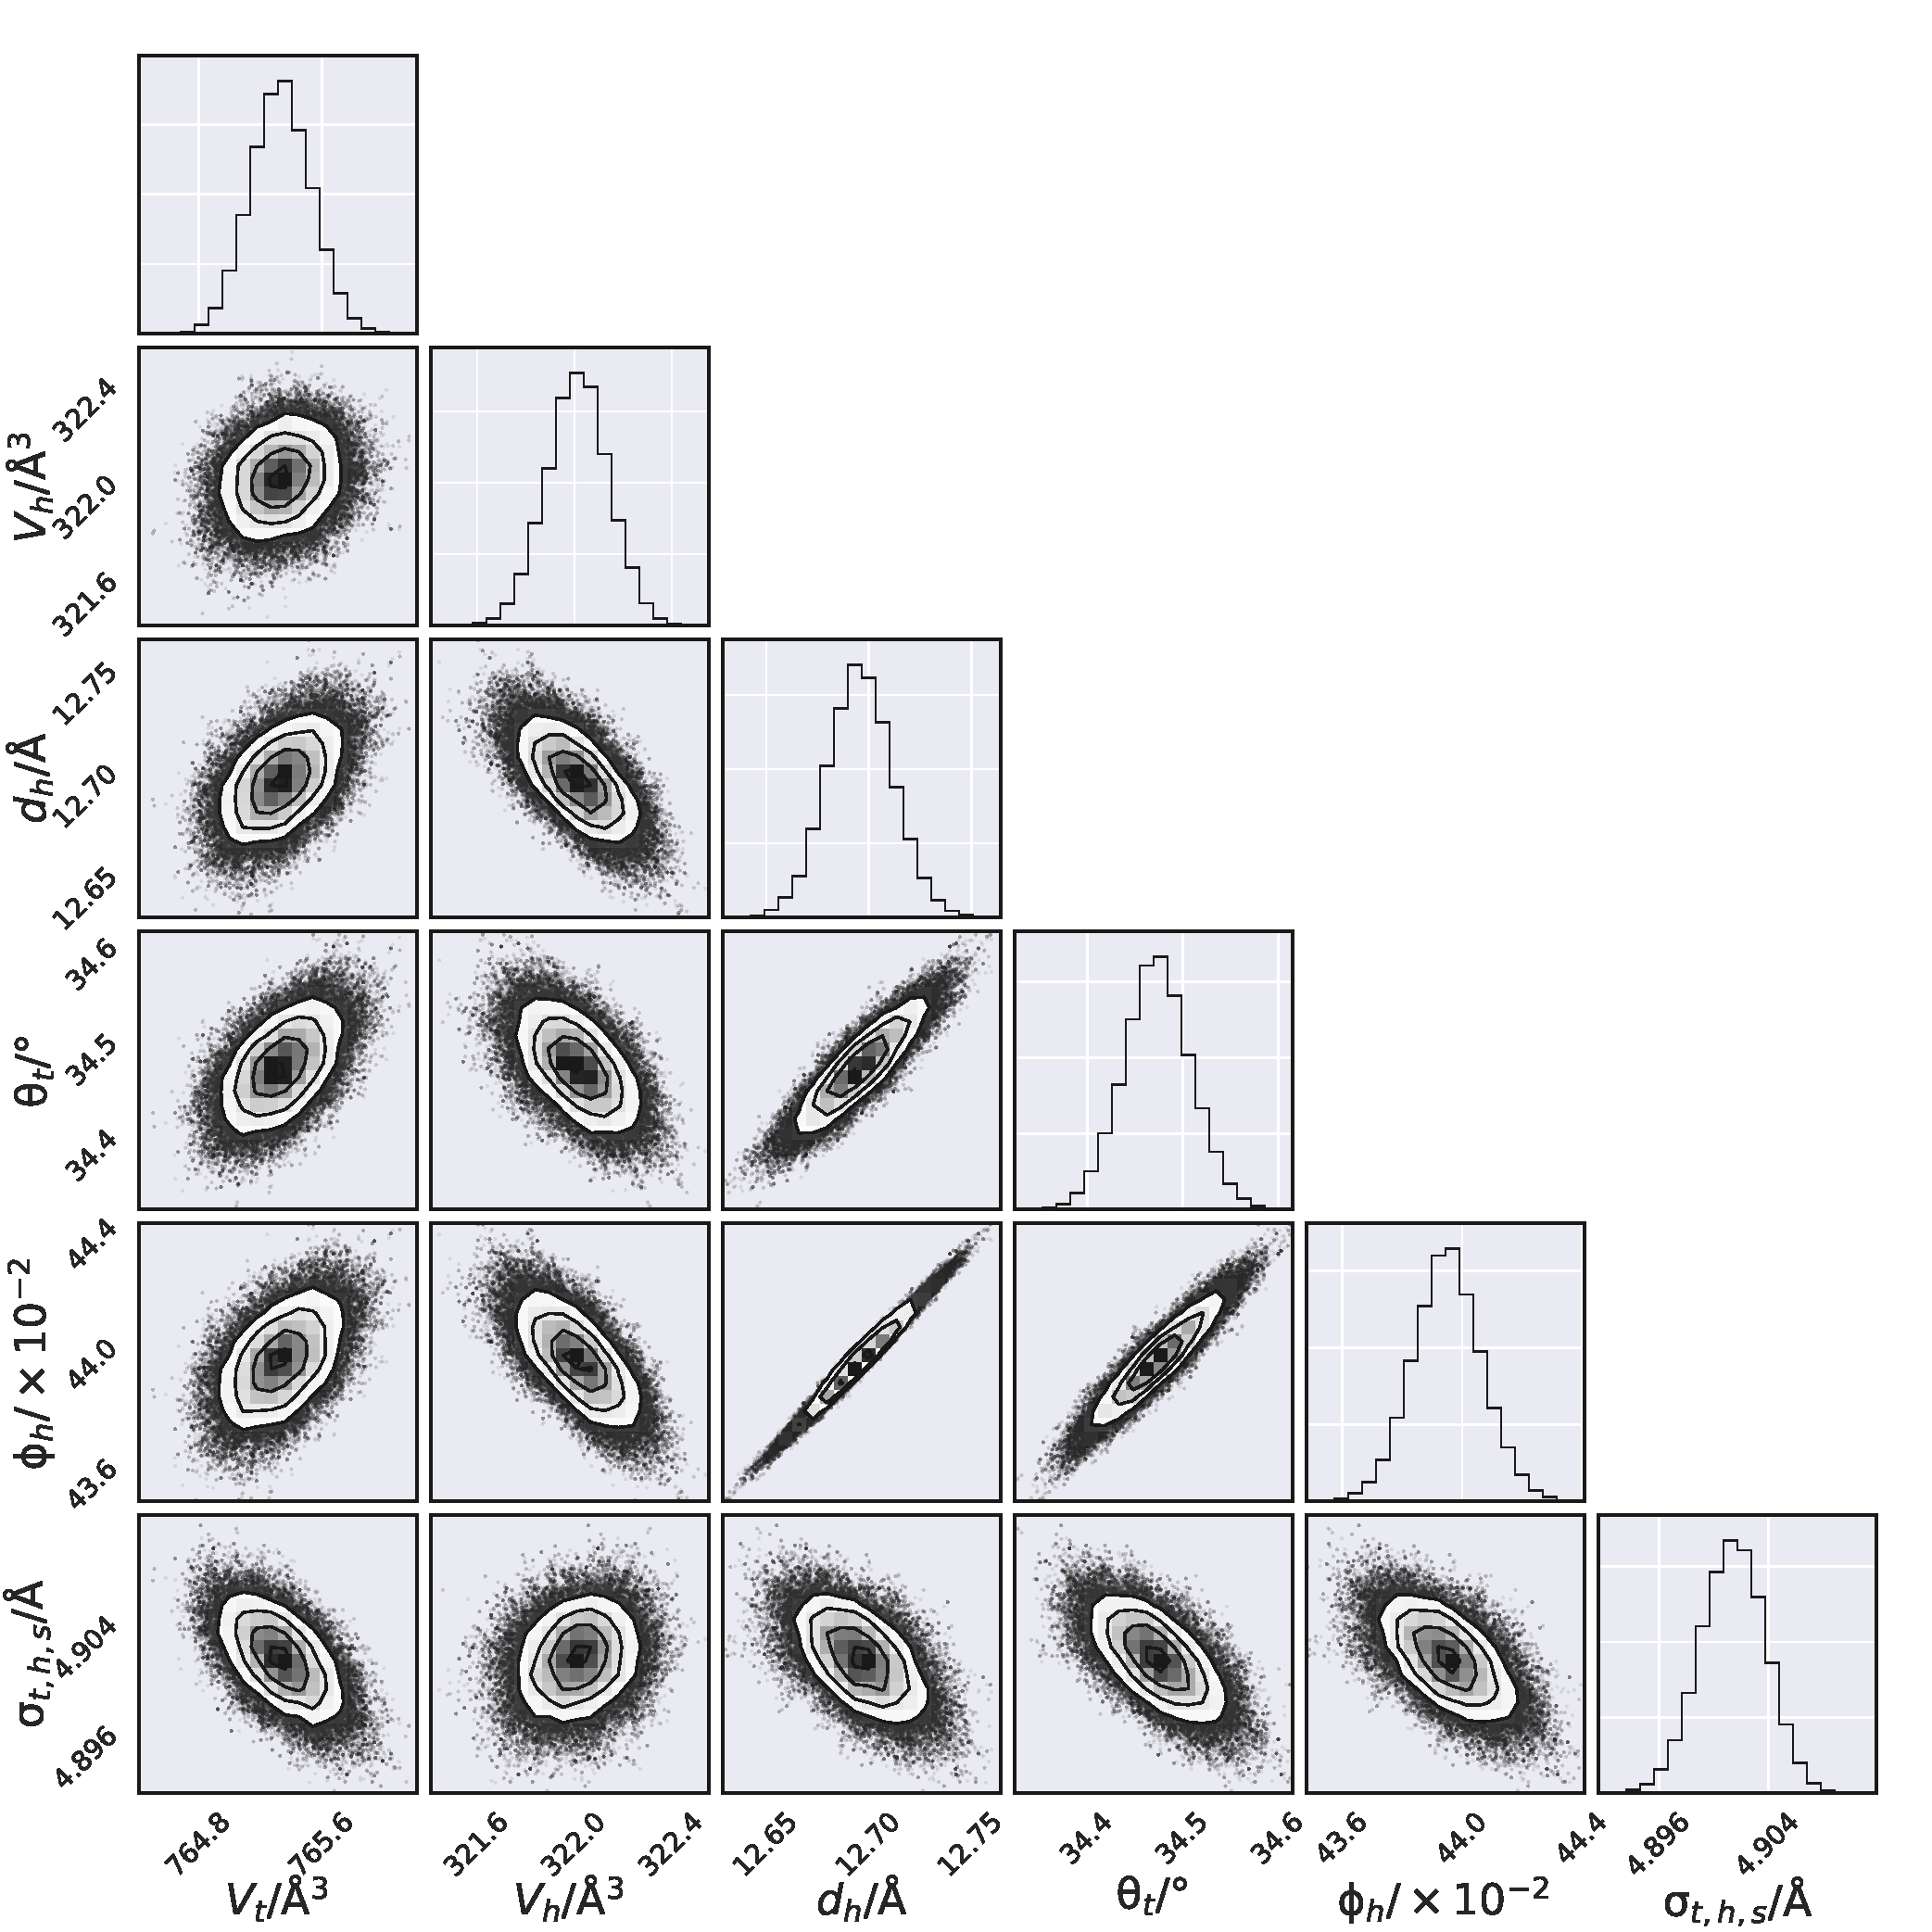
\includegraphics[width=0.50\textwidth]{figures/dppc5_all_corner}
	\caption{The multi-parameter PDFs for the chemically-relevant model of DPPC X-ray reflectometry data at 30 mNm$^{-1}$. Source: Datasets, figure files and running/plotting scripts are available under CC-BY.\cite{mccluskey_2018}}
	\label{fig:dppc5}
\end{figure}
\begin{figure}[h]
	\centering
	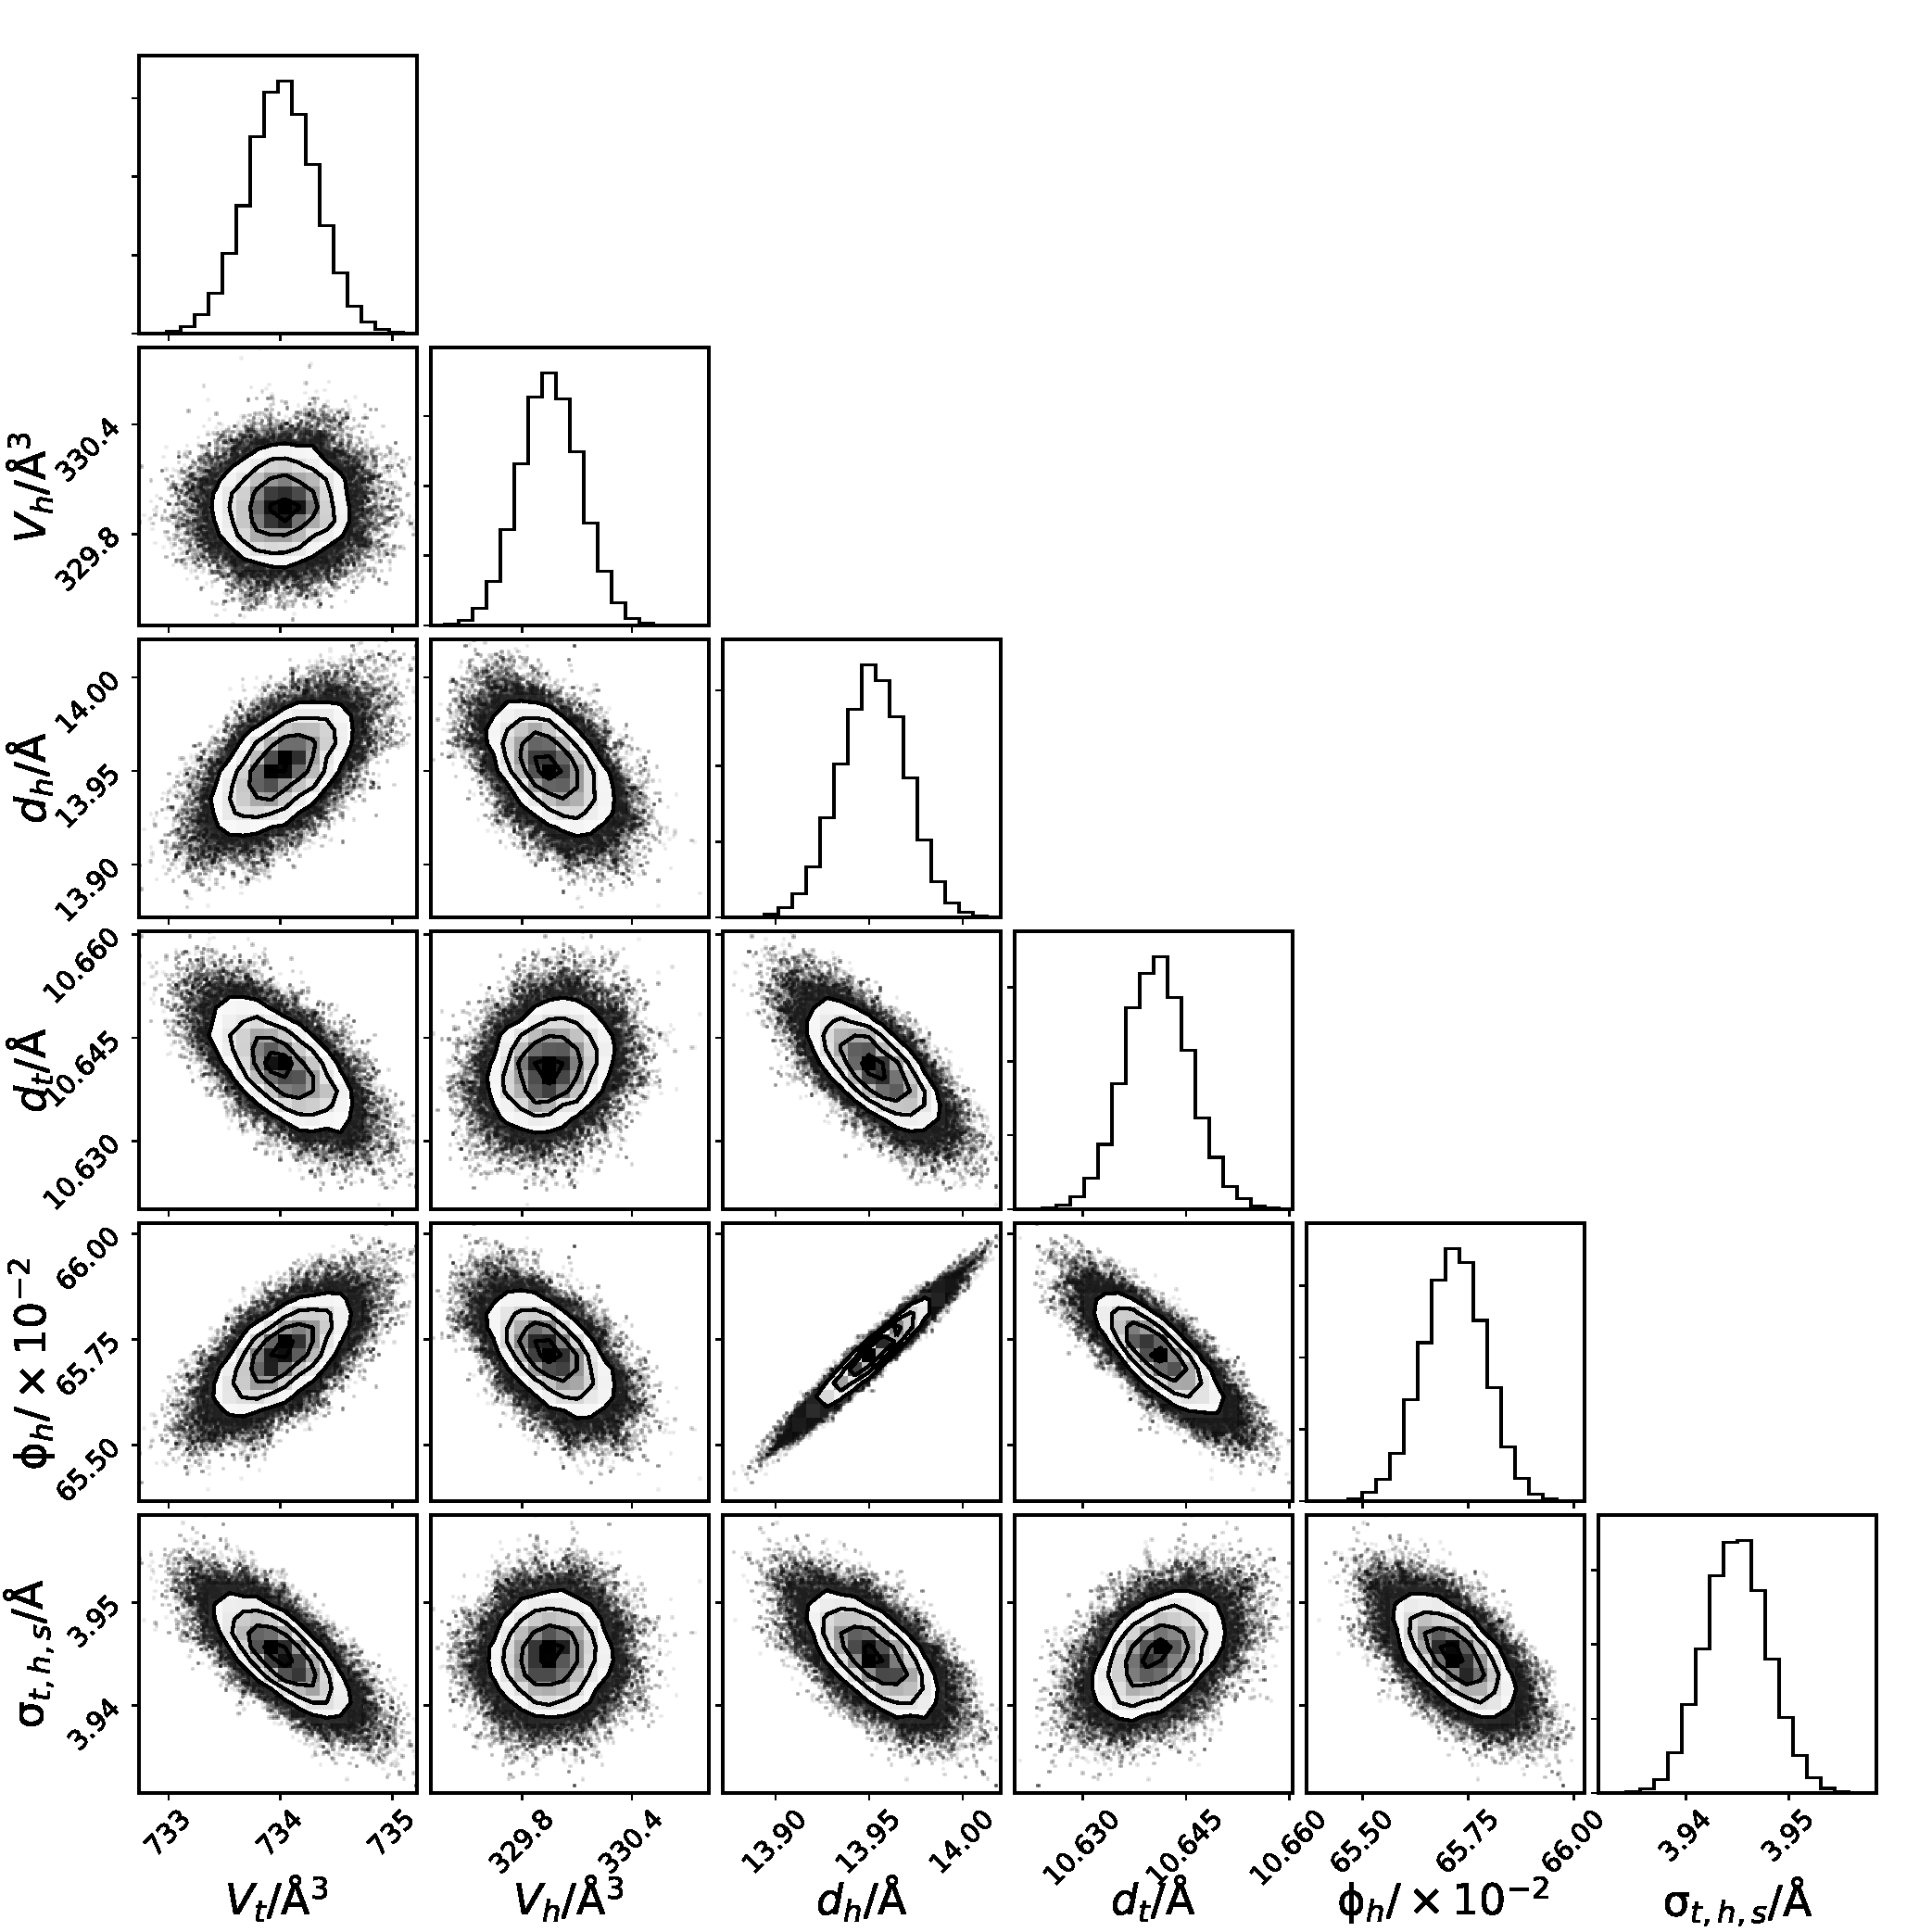
\includegraphics[width=0.50\textwidth]{figures/dmpg2_all_corner}
	\caption{The multi-parameter PDFs for the chemically-relevant model of DMPG X-ray reflectometry data at 15 mNm$^{-1}$. Source: Datasets, figure files and running/plotting scripts are available under CC-BY.\cite{mccluskey_2018}}
	\label{fig:dmpg2}
\end{figure}
\begin{figure}[h]
	\centering
	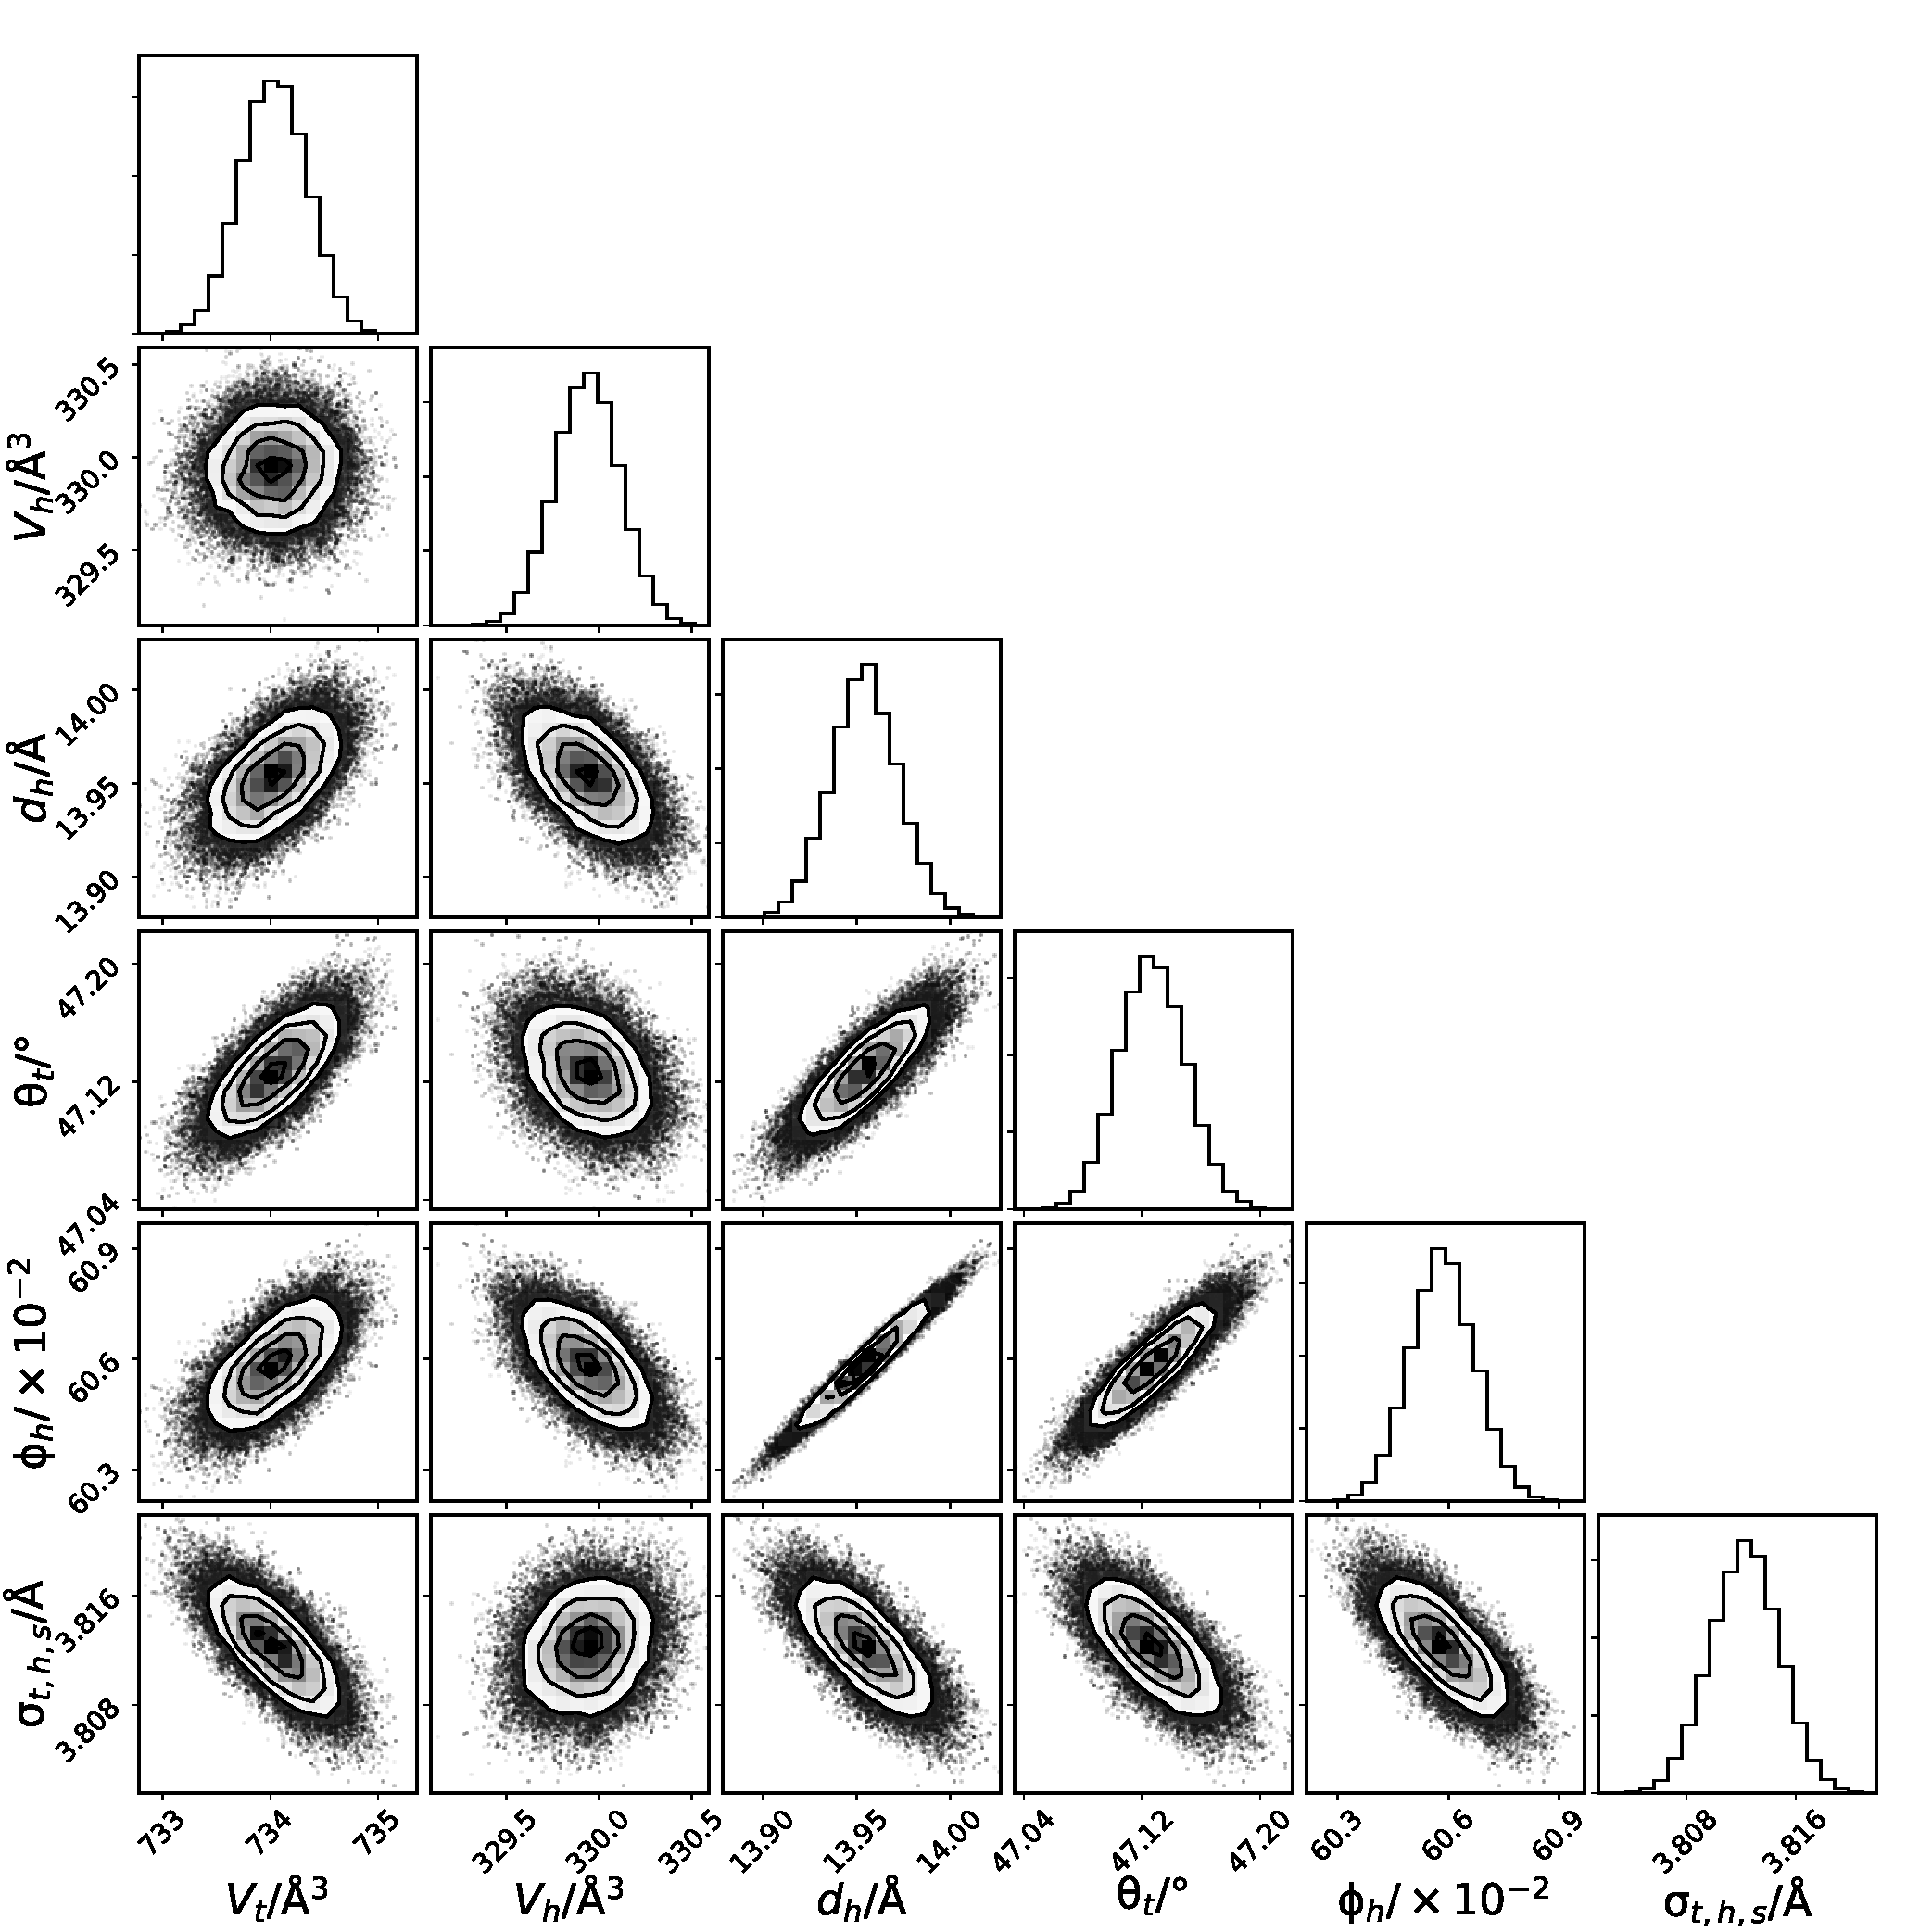
\includegraphics[width=0.50\textwidth]{figures/dmpg3_all_corner}
	\caption{The multi-parameter PDFs for the chemically-relevant model of DMPG X-ray reflectometry data at 20 mNm$^{-1}$. Source: Datasets, figure files and running/plotting scripts are available under CC-BY.\cite{mccluskey_2018}}
	\label{fig:dmpg3}
\end{figure}
\begin{figure}[h]
	\centering
	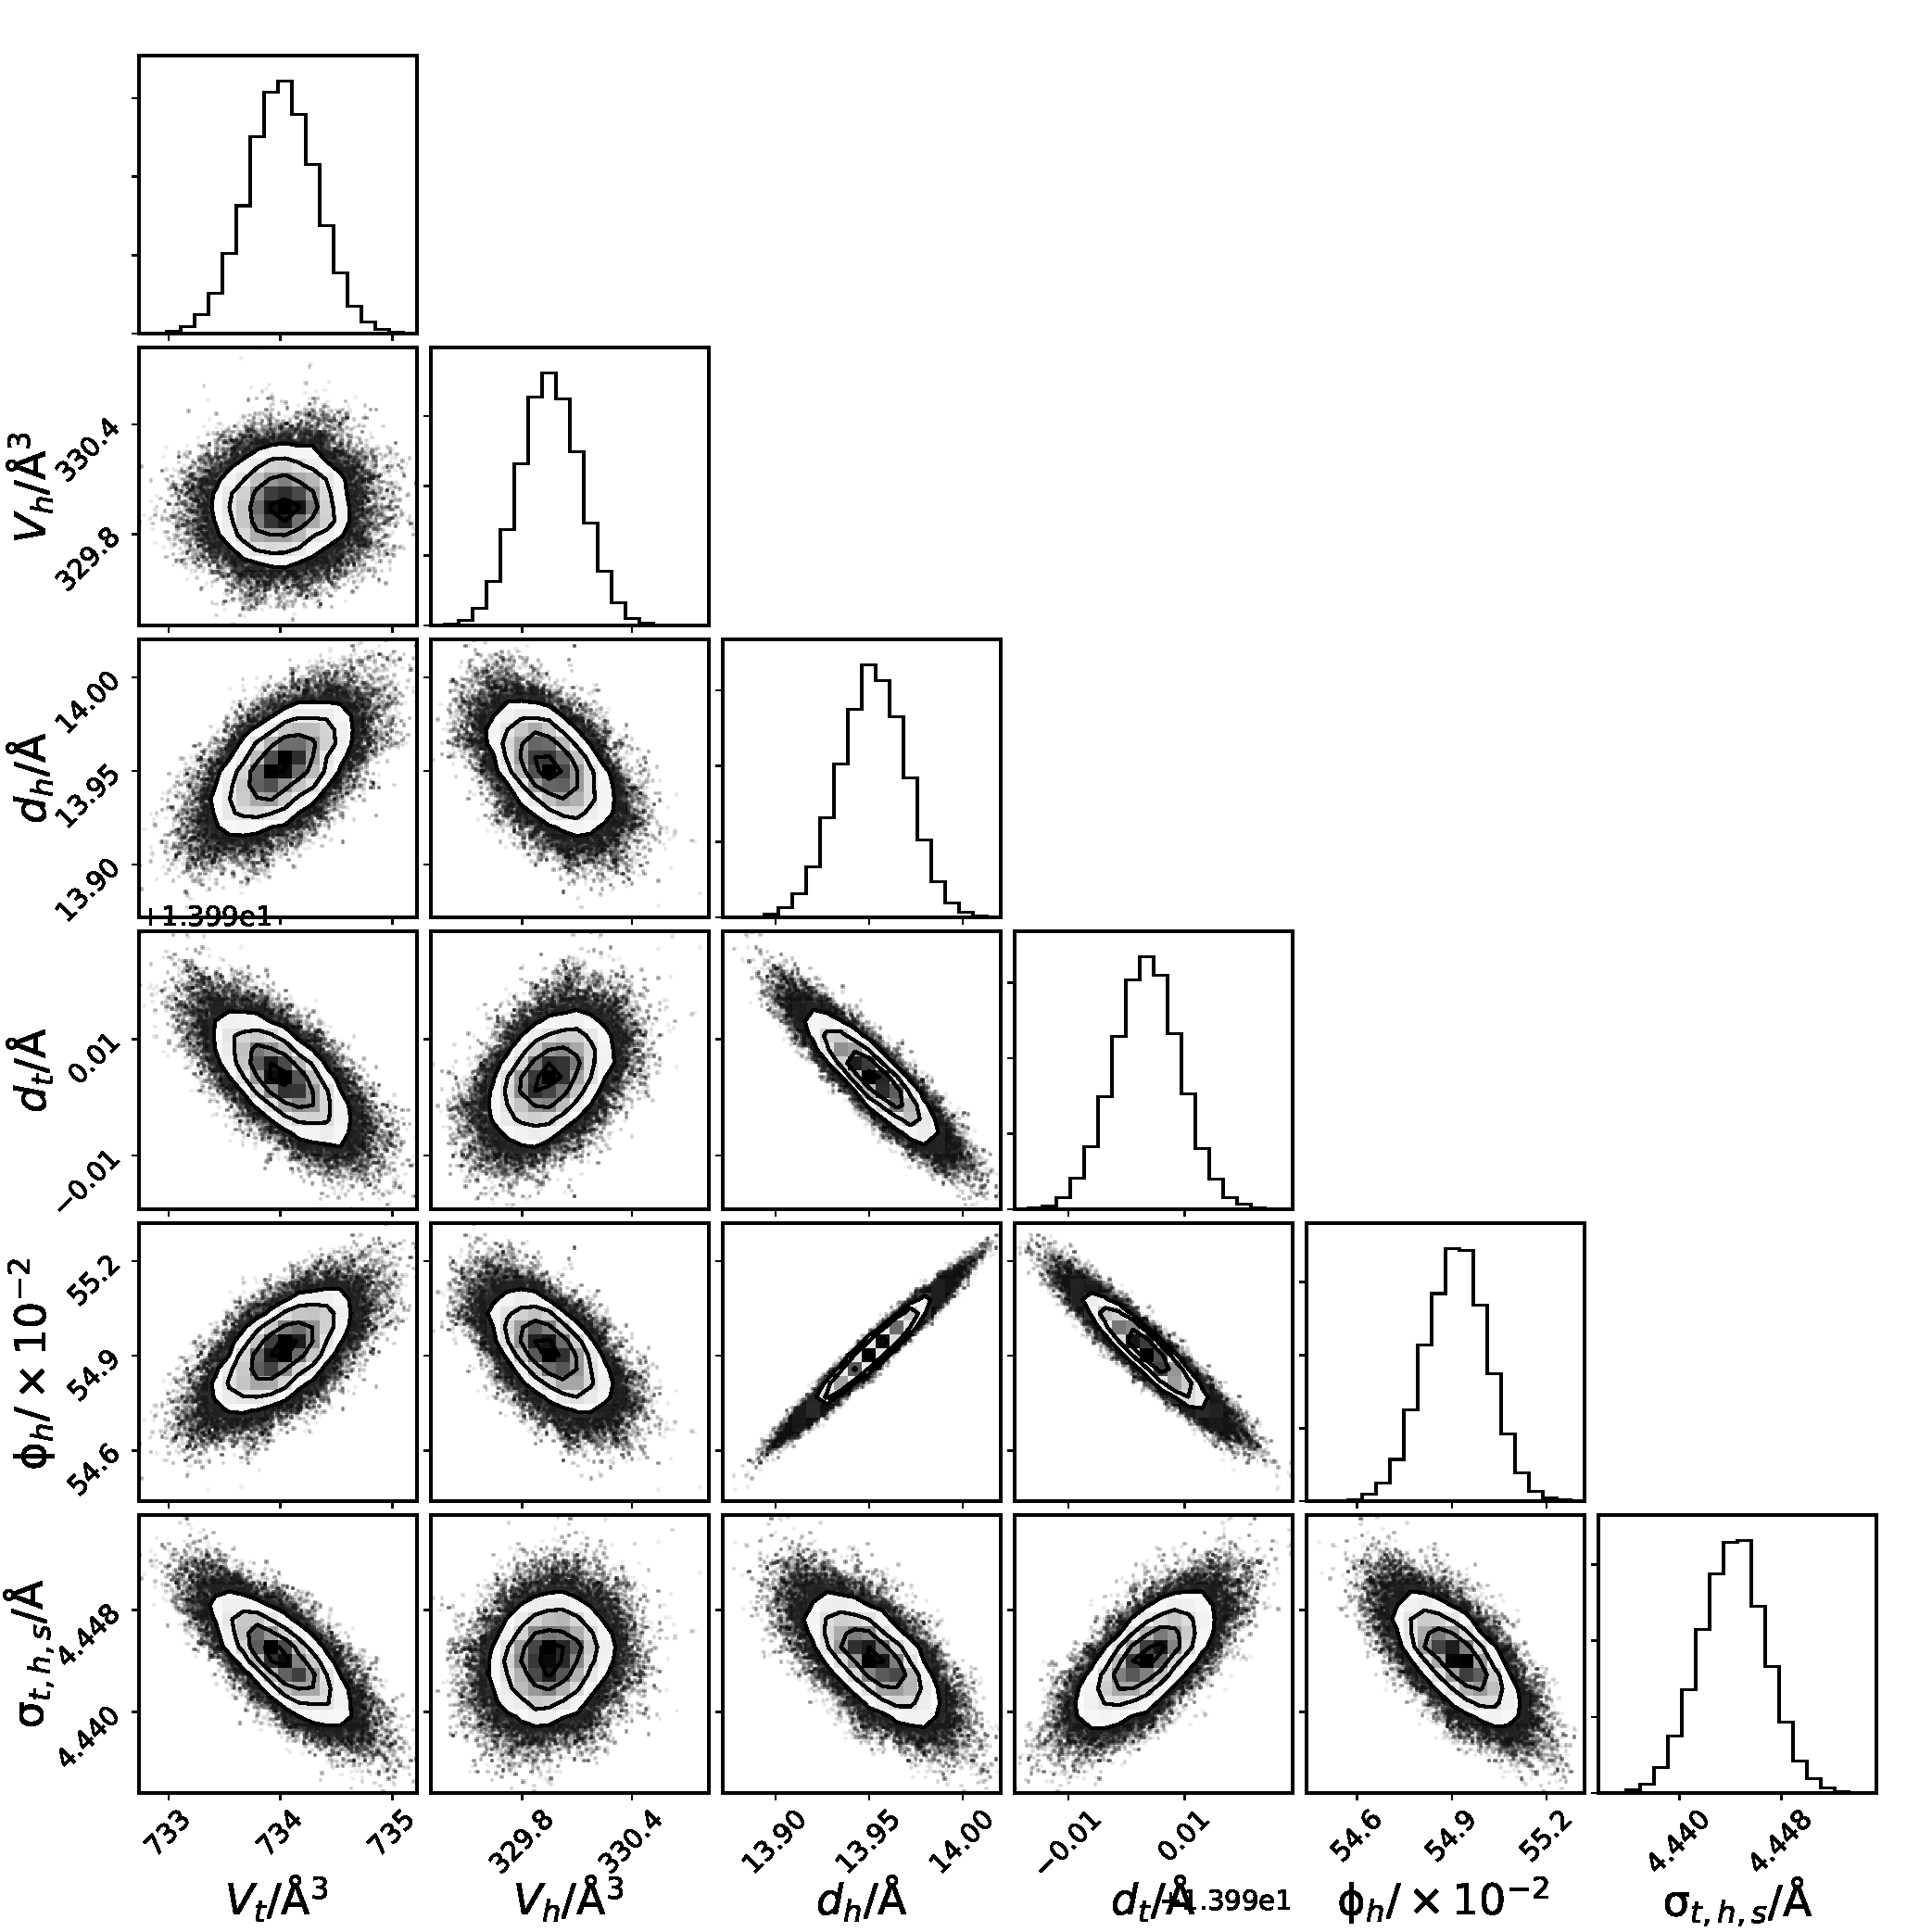
\includegraphics[width=0.50\textwidth]{figures/dmpg4_all_corner}
	\caption{The multi-parameter PDFs for the chemically-relevant model of DMPG X-ray reflectometry data at 25 mNm$^{-1}$. Source: Datasets, figure files and running/plotting scripts are available under CC-BY.\cite{mccluskey_2018}}
	\label{fig:dmpg4}
\end{figure}
\begin{figure}
	\centering
	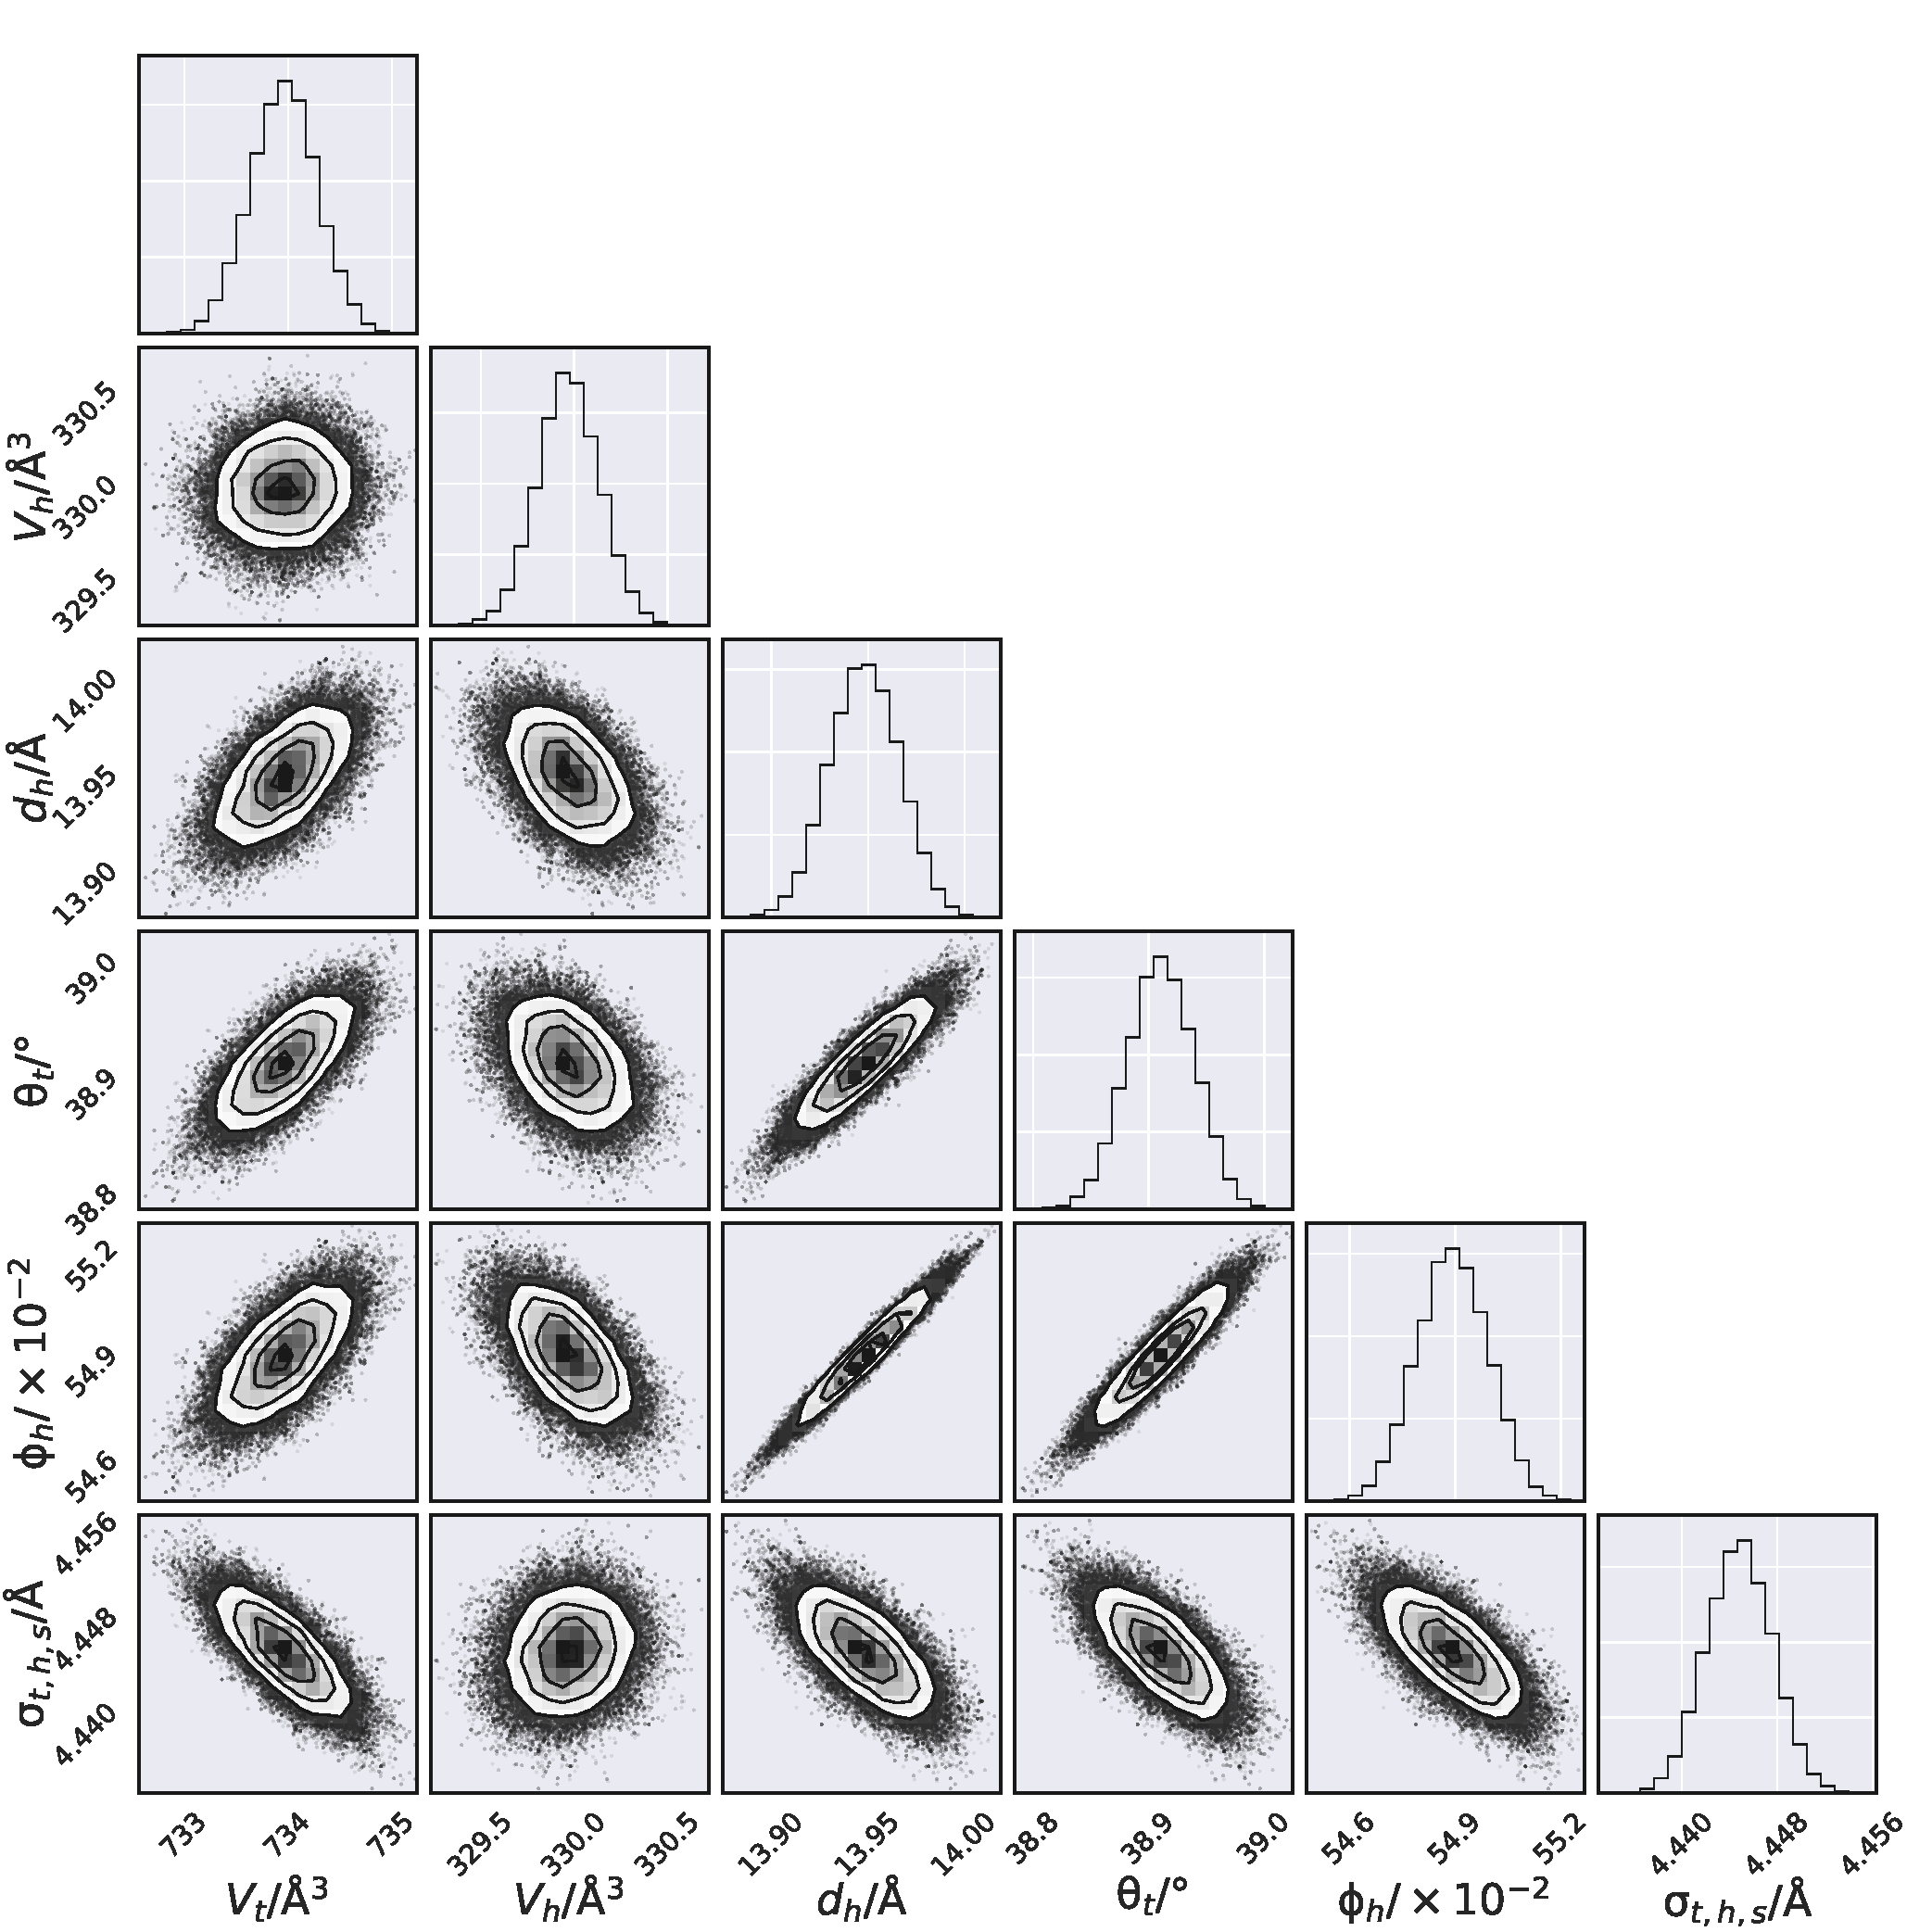
\includegraphics[width=0.50\textwidth]{figures/dmpg5_all_corner}
	\caption{The multi-parameter PDFs for the chemically-relevant model of DMPG X-ray reflectometry data at 30 mNm$^{-1}$. Source: Datasets, figure files and running/plotting scripts are available under CC-BY.\cite{mccluskey_2018}}
	\label{fig:dmpg5}
\end{figure}
\begin{figure}[h]
	\centering
	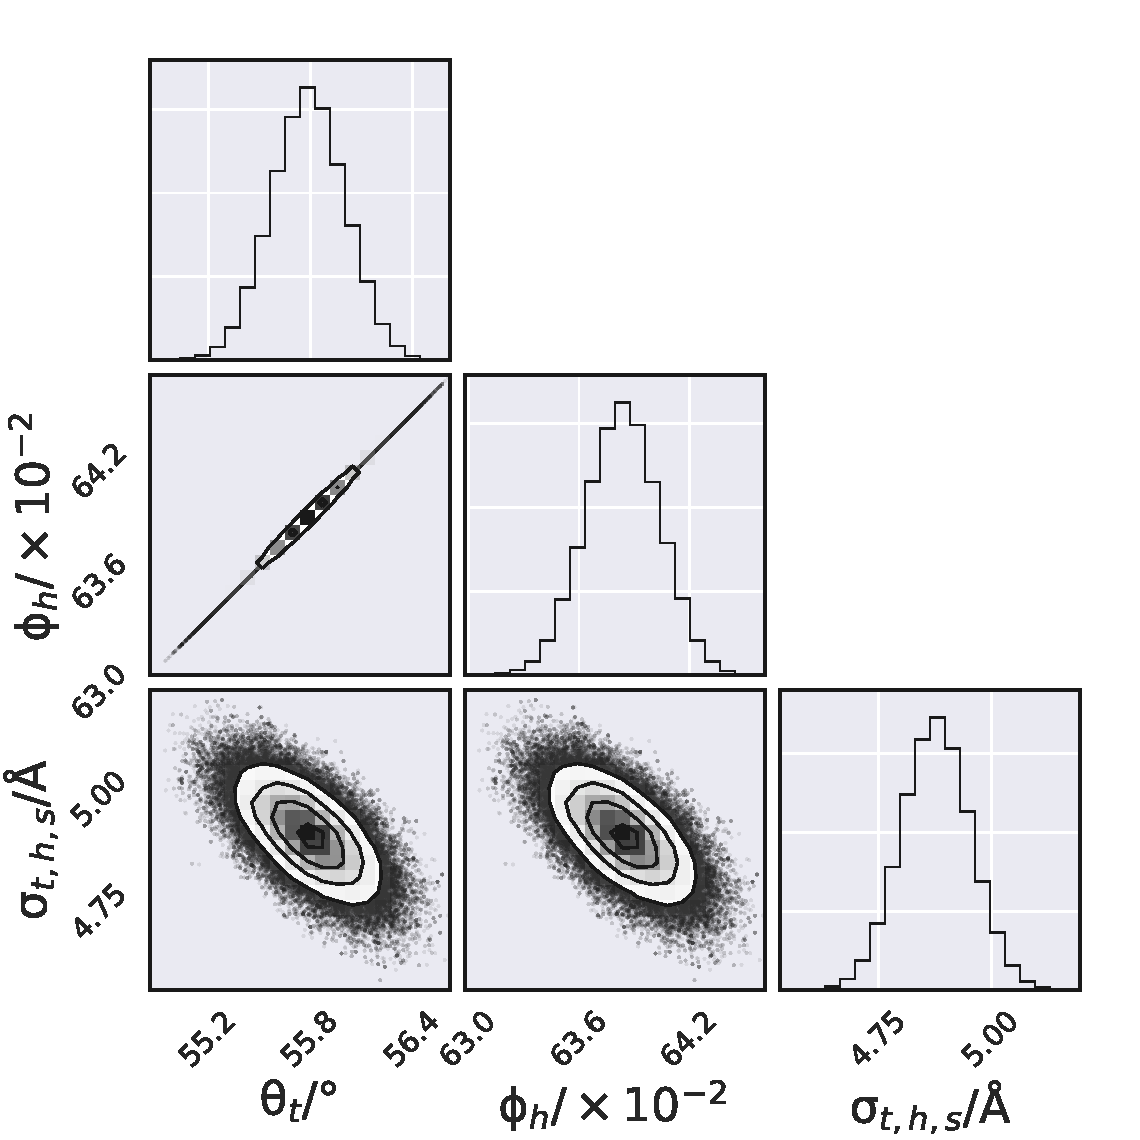
\includegraphics[width=0.50\textwidth]{figures/dmpc20_neutron_corner}
	\caption{The multi-parameter PDFs for the chemically-relevant model of two contrast DMPC neutron reflectometry data at 20 mNm$^{-1}$. Source: Datasets, figure files and running/plotting scripts are available under CC-BY.\cite{mccluskey_2018}}
	\label{fig:dmpcn1}
\end{figure}
\begin{figure}[h]
	\centering
	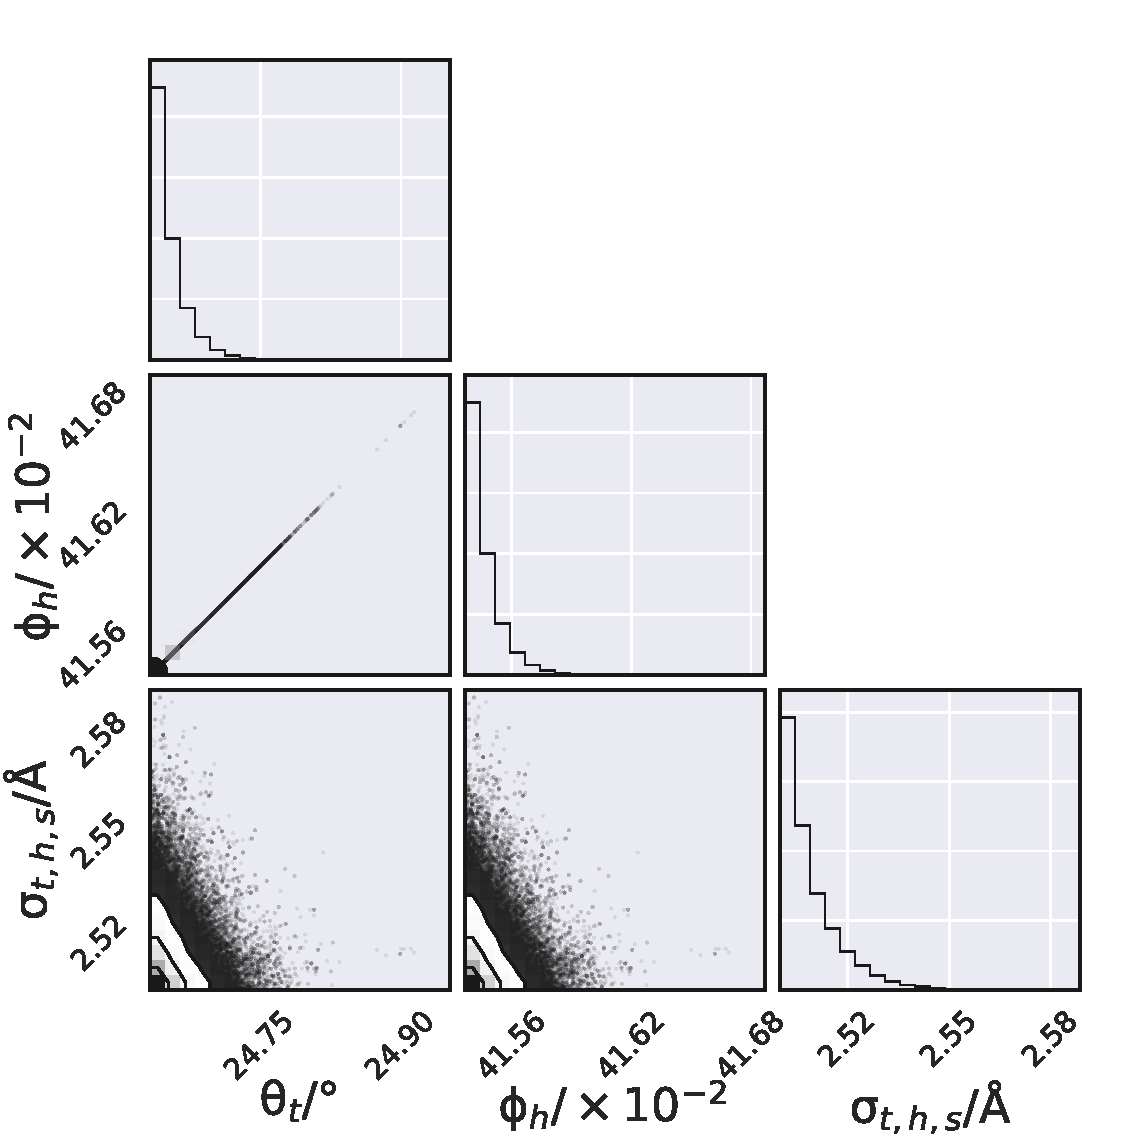
\includegraphics[width=0.50\textwidth]{figures/dmpc25_neutron_corner}
	\caption{The multi-parameter PDFs for the chemically-relevant model of two contrast DMPC neutron reflectometry data at 25 mNm$^{-1}$. Source: Datasets, figure files and running/plotting scripts are available under CC-BY.\cite{mccluskey_2018}}
	\label{fig:dmpcn2}
\end{figure}
\begin{figure}[h]
	\centering
	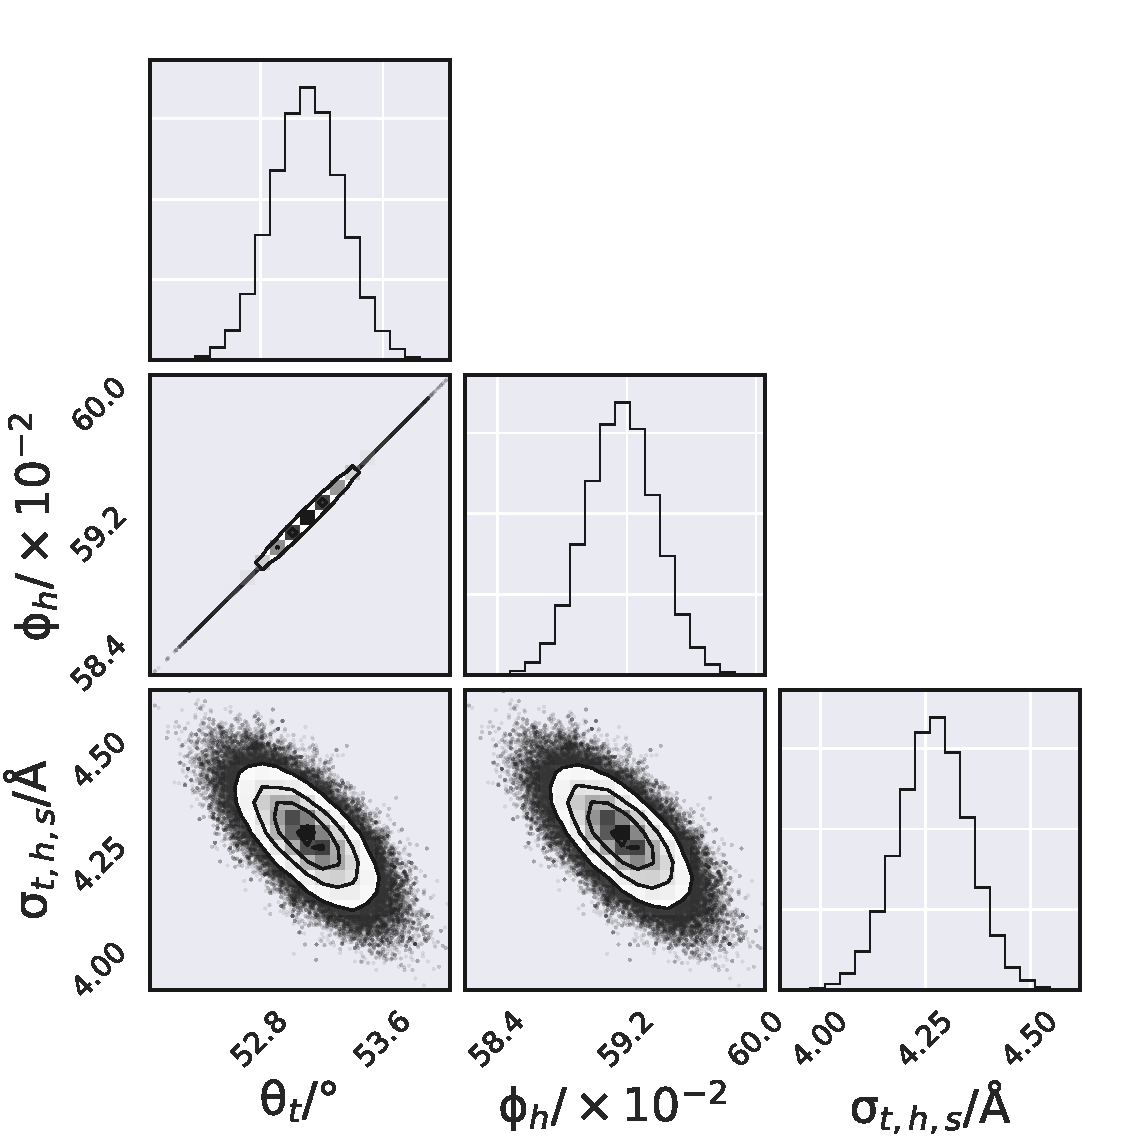
\includegraphics[width=0.50\textwidth]{figures/dppc15_neutron_corner}
	\caption{The multi-parameter PDFs for the chemically-relevant model of two contrast DPPC neutron reflectometry data at 15 mNm$^{-1}$. Source: Datasets, figure files and running/plotting scripts are available under CC-BY.\cite{mccluskey_2018}}
	\label{fig:dppcn1}
\end{figure}
\begin{figure}[h]
	\centering
	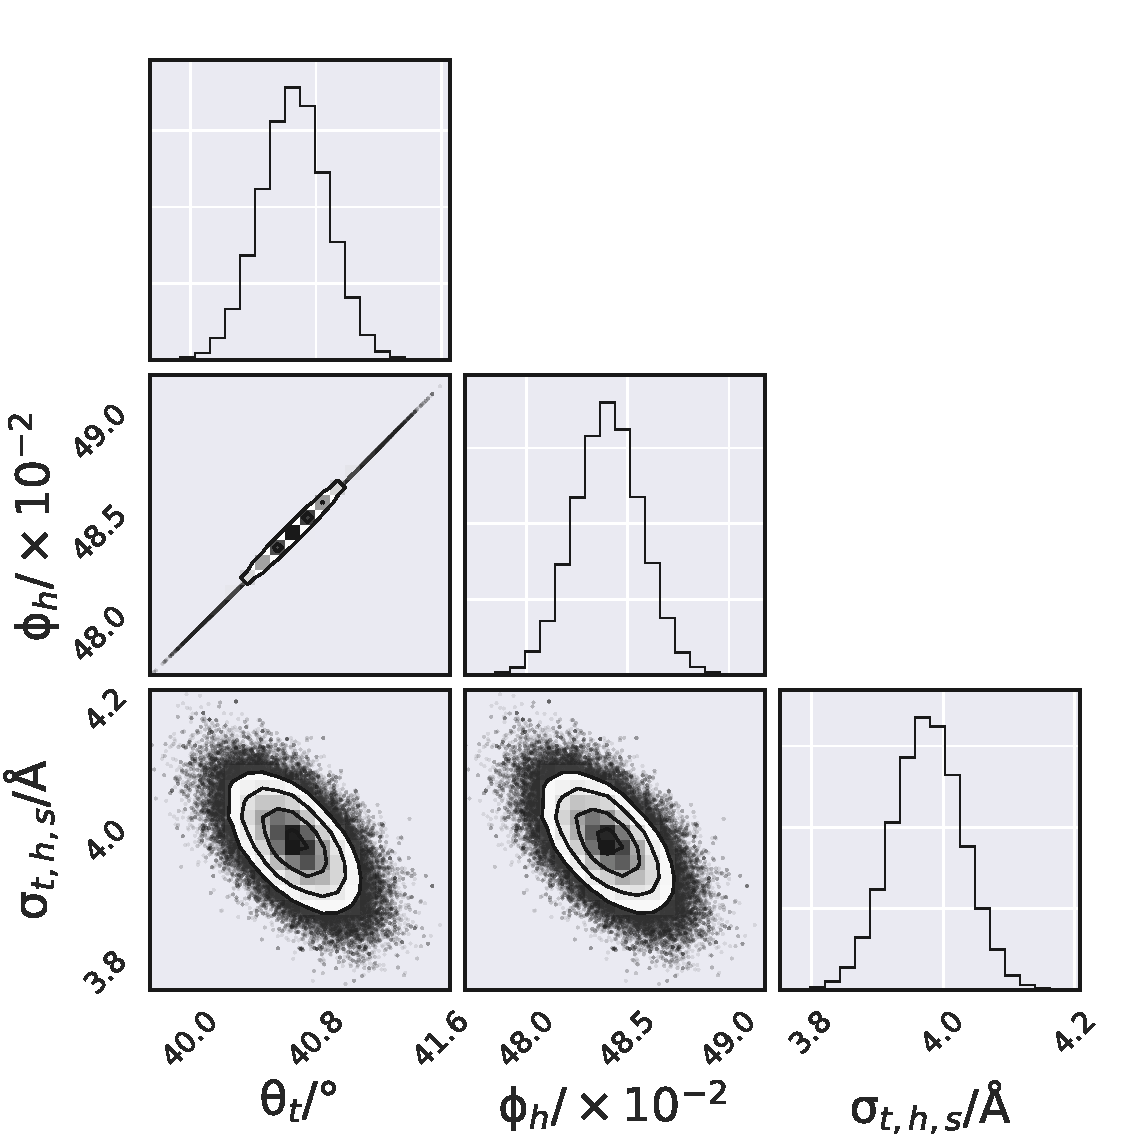
\includegraphics[width=0.50\textwidth]{figures/dppc20_neutron_corner}
	\caption{The multi-parameter PDFs for the chemically-relevant model of two contrast DMPC neutron reflectometry data at 20 mNm$^{-1}$. Source: Datasets, figure files and running/plotting scripts are available under CC-BY.\cite{mccluskey_2018}}
	\label{fig:dppcn2}
\end{figure}

%%%REFERENCES%%%
\bibliography{rsc} %You need to replace "rsc" on this line with the name of your .bib file
\bibliographystyle{rsc} %the RSC's .bst file
\end{document}
